\section{Introduction}\label{introduction}

Drilling rigs are energy-intensive industrial systems whose electrical
demand changes sharply with operating state. Drilling, circulation,
connection, tripping, and auxiliary activities impose different demand
levels and different transition dynamics. When a rig is supplied by a
weak grid connection, diesel generator units, and a battery energy
storage system (BESS), the operating problem involves more than reducing
energy cost. The controller must also maintain power balance, respect
generator commitment and ramping constraints, preserve sufficient
storage state of charge (SOC), and protect high-priority loads when
available supply becomes insufficient.

This problem has a direct operational consequence. A controller that
reacts only to instantaneous load may discharge the BESS before a
transition, or may start too many diesel units and replace relatively
inexpensive grid power with fuel consumption. Conversely, a controller
that focuses only on economic dispatch may leave insufficient reserve
for a short high-power event. The resulting trade-off is particularly
important for drilling rigs because their load profile combines
sustained operation with short, high-amplitude transitions.

Energy management studies have investigated hierarchical scheduling,
multi-objective microgrid dispatch, energy storage coordination, and
model predictive control (MPC). For example, bilevel energy management
has been used to coordinate security, reliability, storage, and
demand-side management
\citep{jokar2022bilevel},
while predictive energy management has been applied to hybrid vessel
grids \citep{vafamand2020predictive}. Stochastic and random-setting formulations have also been used
for isolated hybrid microgrids with diesel generation and storage
\citep{vergine2022optimal}.
These studies establish the value of combining forecasting, uncertainty
representation, and constrained optimization. They also motivate a
system-level evaluation that reports drilling-load transitions, discrete
multi-generator commitment, storage protection, and emergency load
prioritization under one declared protocol.

The closest drilling rig precedent considered rule-based generator
scheduling together with battery storage for diesel power-plant
fuel-efficiency improvement
\citep{pavkovic2016oil}. This prior work motivates the present application, but it also
sets a clear comparison requirement: the contribution cannot be reduced
to using a BESS in a drilling rig. The relevant question is whether
forecast uncertainty and supply risk can be transferred into a
controller that remains feasible under the stated active-power constraints while avoiding unnecessary
generator commitment.

This paper evaluates a reserve--SOC supervisory energy-management framework
for a grid--diesel--battery drilling rig power system. The systems question is
whether storage reserve and model-reachable generator capacity can be coordinated
early enough, using only causal forecast information, to reduce shortage during
abrupt load transitions. The framework links short-horizon forecast scenarios
to conditional value-at-risk (CVaR) dispatch, discrete generator commitment,
SOC hysteresis, and priority-based load protection. The individual ingredients
are established in prior work. The contribution claimed here is a
system-specific supervisory coupling whose mechanism and operating effects are
tested under a common causal and physical boundary. The paper makes three
contributions:

\begin{enumerate}
\def\labelenumi{\arabic{enumi}.}
\tightlist
\item
  We design and implement a reserve--SOC supervisor that combines a causal
  forecast envelope, current SOC, and model-reachable generator capacity within a
  receding-horizon grid--diesel--battery dispatch model.
\item
  We evaluate the controller under a prospectively frozen 12-seed simulation
  protocol against rule-based and matched MILP references, with validation-only
  residual scenarios, seed-level inference, component interventions, and
  constraint audits that separate reliability from operating-cost effects.
\item
  We add a multi-source public-data checking layer based on real
  measurements: two drilling-process records, eight electrical-load series,
  and two BESS operating records. This layer tests forecast transfer, storage
  behavior, and simulator assumptions without relabeling those data as
  target-rig closed-loop evidence.
\end{enumerate}

The controller comparison uses 72 h simulated replays. The revised dispatch
protocol declares a new seed queue and retains the first 12 upstream-eligible
holdouts; previously inspected seeds are development-only. Public real data
provide external evidence for selected inputs and physical relationships, but
no public source contains synchronized target-rig bus power and supply-side
states suitable for a closed-loop replay. The controller-efficacy claim
therefore remains simulation-bounded. Section~\ref{system-boundary-and-data}
describes the evidence roles and their boundaries.

\section{Related work}\label{related-work}

\subsection{Drilling-rig storage and load-shock control}

Storage is not new to drilling-rig power systems. Pavkovi\'{c} et al. combined
rule-based generator scheduling with a battery energy storage system (BESS) to
improve diesel-plant operation under drilling loads
\citep{pavkovic2016oil}. Chupin et al. reviewed the associated sizing and
operating problem \citep{chupin2021drillingstorage}, while Huang et al.
considered offshore scheduling under uncertain renewable generation and
platform demand \citep{huang2019drilling}. More recently, Wang et al. proposed
operating-state-dependent dual power allocation and converter-level control
for an electrified oil rig, and evaluated the system with full-cycle field
power and operating records \citep{wang2025dualpower}. That field evidence is
stronger than the simulation evidence available in the present study. Our
narrower question is whether validation-calibrated forecast-error scenarios,
model-reachable multi-unit commitment, and SOC reserve supervision improve
constraint-feasible active-power dispatch when all alternatives share one
causal replay and plant model.

\subsection{Closest predictive-dispatch precedents}

The closest precedent is the stochastic economic MPC of Chapaloglou et al.,
which combines data-driven uncertainty scenarios with mixed-integer unit
scheduling for an isolated oil-and-gas power system subject to abrupt,
irregular loads \citep{chapaloglou2022datadriven}. Moretti et al. studied a
two-layer predictive dispatch algorithm using field data from an off-grid
microgrid \citep{moretti2019twolayer}; Nelson and Johnson demonstrated
real-time microgrid MPC for ancillary-service participation
\citep{nelson2020realtime}. These studies establish both the stochastic-MPC
precedent and stronger routes to field or experimental validation. The present
study differs in its drilling-load replay, grid--diesel--battery topology,
5-s receding-horizon update, explicit generator reachability, and SOC reserve
supervisor. Its main methodological control is a matched ablation: persistence,
point-forecast, fixed-reserve, residual-CVaR, risk-adaptive, and full
supervisory variants execute through the same dispatch implementation and use
the same terminal-SOC rule. Because the plants and data differ, we do not claim
head-to-head superiority over the cited systems.

\subsection{Uncertainty, reserve, and supervisory MPC}

Predictive energy management for microgrids is well established
\citep{hu2021mpcoverview,abbasi2023emsreview}. Relevant formulations include
resilience-oriented multi-scenario reserve control
\citep{tobajas2022resilience}, stochastic MILP
\citep{franke2020stochasticmilp}, and robust cost--risk scheduling with CVaR
\citep{ji2018robustcvar}. We use the auxiliary-threshold CVaR formulation of
Rockafellar and Uryasev \citep{rockafellar2000cvar}, but treat it as a standard
ingredient rather than a contribution. The study-specific additions are:
(i) full-horizon residual trajectories drawn only from validation data;
(ii) a finite-scenario tail-resolution gate that prevents a nominal confidence
level from collapsing onto too few scenarios; (iii) risk-conditioned reserve
and commitment supervision; and (iv) separate reporting of operating cost,
terminal-energy adjustment, and reliability penalty. Priority-based load
allocation is retained only as a shortage diagnostic; it is not evidence that
total supply adequacy has improved.

\subsection{Forecasting role and evidence boundary}

The forecasting stage compares naive, tree-based, recurrent, convolutional,
and transformer-based candidates. Temporal Fusion Transformer, PatchTST, and
iTransformer provide relevant attention-based forecasting precedents
\citep{lim2021tft,nie2023patchtst,liu2024itransformer}; the implemented candidate
set and selection rule are stated explicitly in
Sections~\ref{forecasting-module} and~\ref{baselines}.
These models are baselines, not the claimed novelty. The controller is evaluated
by causal simulation replay, whereas Wang et al., Moretti et al., and Nelson
and Johnson provide field or experimental controller evidence
\citep{wang2025dualpower,moretti2019twolayer,nelson2020realtime}. We use public
real measurements for three bounded external checks: drilling-process timing,
cross-domain electrical-load forecasting, and BESS power--SOC behavior. The
drilling records lack synchronized rig-bus active power and supply-side state,
and the electrical and storage records are not from the target rig. Accordingly,
the paper claims simulation-based controller efficacy plus bounded real-data
component and assumption checks; it does not claim deployment readiness,
voltage/frequency stability, converter-level performance, or target-rig field
generalization. Within that boundary, the contribution is the controlled
comparison of how causally calibrated forecast uncertainty, discrete
commitment, and SOC supervision interact under rapid load transitions.

Table~\ref{tab:closest-capabilities} makes the comparison boundary explicit.
``Not reported'' means that the cited article does not use that element as a
reported evaluation feature; it is not a judgment that the element could not be
added to the method.

\begin{table}[!t]
\caption{Capability comparison with the closest application and predictive-dispatch precedents}
\label{tab:closest-capabilities}
\centering
\scriptsize
\setlength{\tabcolsep}{3pt}
\begin{tabular}{@{}p{2.8cm}ccccp{2.1cm}@{}}
\toprule
Study & Rig / O\&G & Abrupt load & Uncertainty & Multi-unit UC & Evidence \\
\midrule
Pavkovi\'{c} et al. \citep{pavkovic2016oil} & rig & yes & no & rule-based & simulation \\
Wang et al. \citep{wang2025dualpower} & rig & yes & no & not reported & field records \\
Chapaloglou et al. \citep{chapaloglou2022datadriven} & O\&G & yes & stochastic & yes & simulation \\
Moretti et al. \citep{moretti2019twolayer} & no & variation & forecast & not reported & field data \\
Nelson and Johnson \citep{nelson2020realtime} & no & market & forecast & not reported & experiment \\
Present study & rig simulation & yes & residual scenarios & four units & simulation plus public real-data external checks \\
\bottomrule
\end{tabular}
\end{table}

\section{System boundary and data}\label{system-boundary-and-data}

\subsection{System boundary}\label{system-boundary}

The system contains four functional components: (i) an external grid
connection with time-varying available capacity, (ii) a set of diesel
generator units, (iii) a BESS with power and SOC limits, and (iv) an
electrical load representing the drilling rig and auxiliary equipment.
The controller receives measurements and causally available state
information. It produces a receding-horizon plan and applies the first
control action before the next measurement update.

The plant is a quasi-static active-power and energy model. It represents source
availability, unit commitment, minimum stable output, ramping, start
synchronization delay, storage energy and SOC-dependent power limits, but not
reactive power, bus voltage, frequency dynamics, short-circuit strength,
protection coordination, converter electromagnetic dynamics, or sub-5-s
transients. Consequently, ``feasible'' below always means feasible under these
stated model constraints.

The load is partitioned into critical, essential, and interruptible classes
for evaluating priority-based protection when available supply is
insufficient. The class proportions are control-study settings; deployment
values must be approved through the drilling rig's electrical and safety
procedures.

The implementation uses a 5 s sampling interval for the main
high-frequency data path. The forecast task uses a 10 min history to
predict the following 1 min horizon. The dispatch controller operates on
the forecast package and current equipment state; all future true load
and future-derived operation-state flags are excluded from online
features.

\subsection{Evaluation data}\label{evaluation-data}

Table~\ref{tab:datasets} separates the evidence sources and their roles. Each
simulator seed produces a 72 h active-power record at 5 s resolution (51,840
timestamped rows before quality processing). The mechanistic drilling-load and
multi-source power-system simulator records total load, operating state,
available supply, generator status, battery power, and SOC. One prespecified
development seed is used for forecast-model comparison, residual-scenario
calibration, controller debugging, and the pre-freeze runtime gate. It is not
included in the primary controller inference. The primary dispatch evidence
comprises the first 12 upstream-eligible seeds in a queue frozen before any of
their controller outcomes were generated.

The development forecasting replay contains 51,709 samples, of which 51,697
are scored. A fixed chronological split is used for model comparison. The power
scaler is fitted on the training partition; ensemble weights and complete
forecast-residual vectors use the validation partition; and test targets are
excluded from model fitting, calibration, and selection. For each prospective
seed, the same upstream fitting and calibration procedure is rerun before its
dispatch comparison, without changing the frozen hyperparameters or decision
rules.

The public-data collection contains eight dataset families and
ten prepared one-minute electrical series, totaling 13,571,131 timestamps;
12,351,203 (91.01\%) pass the dataset-specific frozen quality rules, and target
values are never imputed. Six REFIT houses and the UCI household record provide
directly measured aggregate active power. The Tsukuba load target is derived
from measured grid import, photovoltaic generation, and battery power rather
than a dedicated load meter. M5BAT and Tsukuba provide real BESS power and SOC
trajectories. Energistics Well B and Utah FORGE Well 58-32 provide independent
drilling-process records; neither contains the synchronized total active power
and supply-side state required for controller replay.

OpenCEM was used during pipeline development and its opened period is retained
as exploratory rather than recycled as a confirmatory holdout. Petrobras 3W is
retained only as a scope audit because its production-well anomaly labels are
not power-system risk labels. These exclusions prevent unrelated real data from
being used to manufacture a nominal field-performance score.

Figures~\ref{fig:load-summary} and~\ref{fig:state-curves} summarize the load
features and representative operating-state curves used to define the
forecasting and dispatch problem.

\begin{figure}
\centering
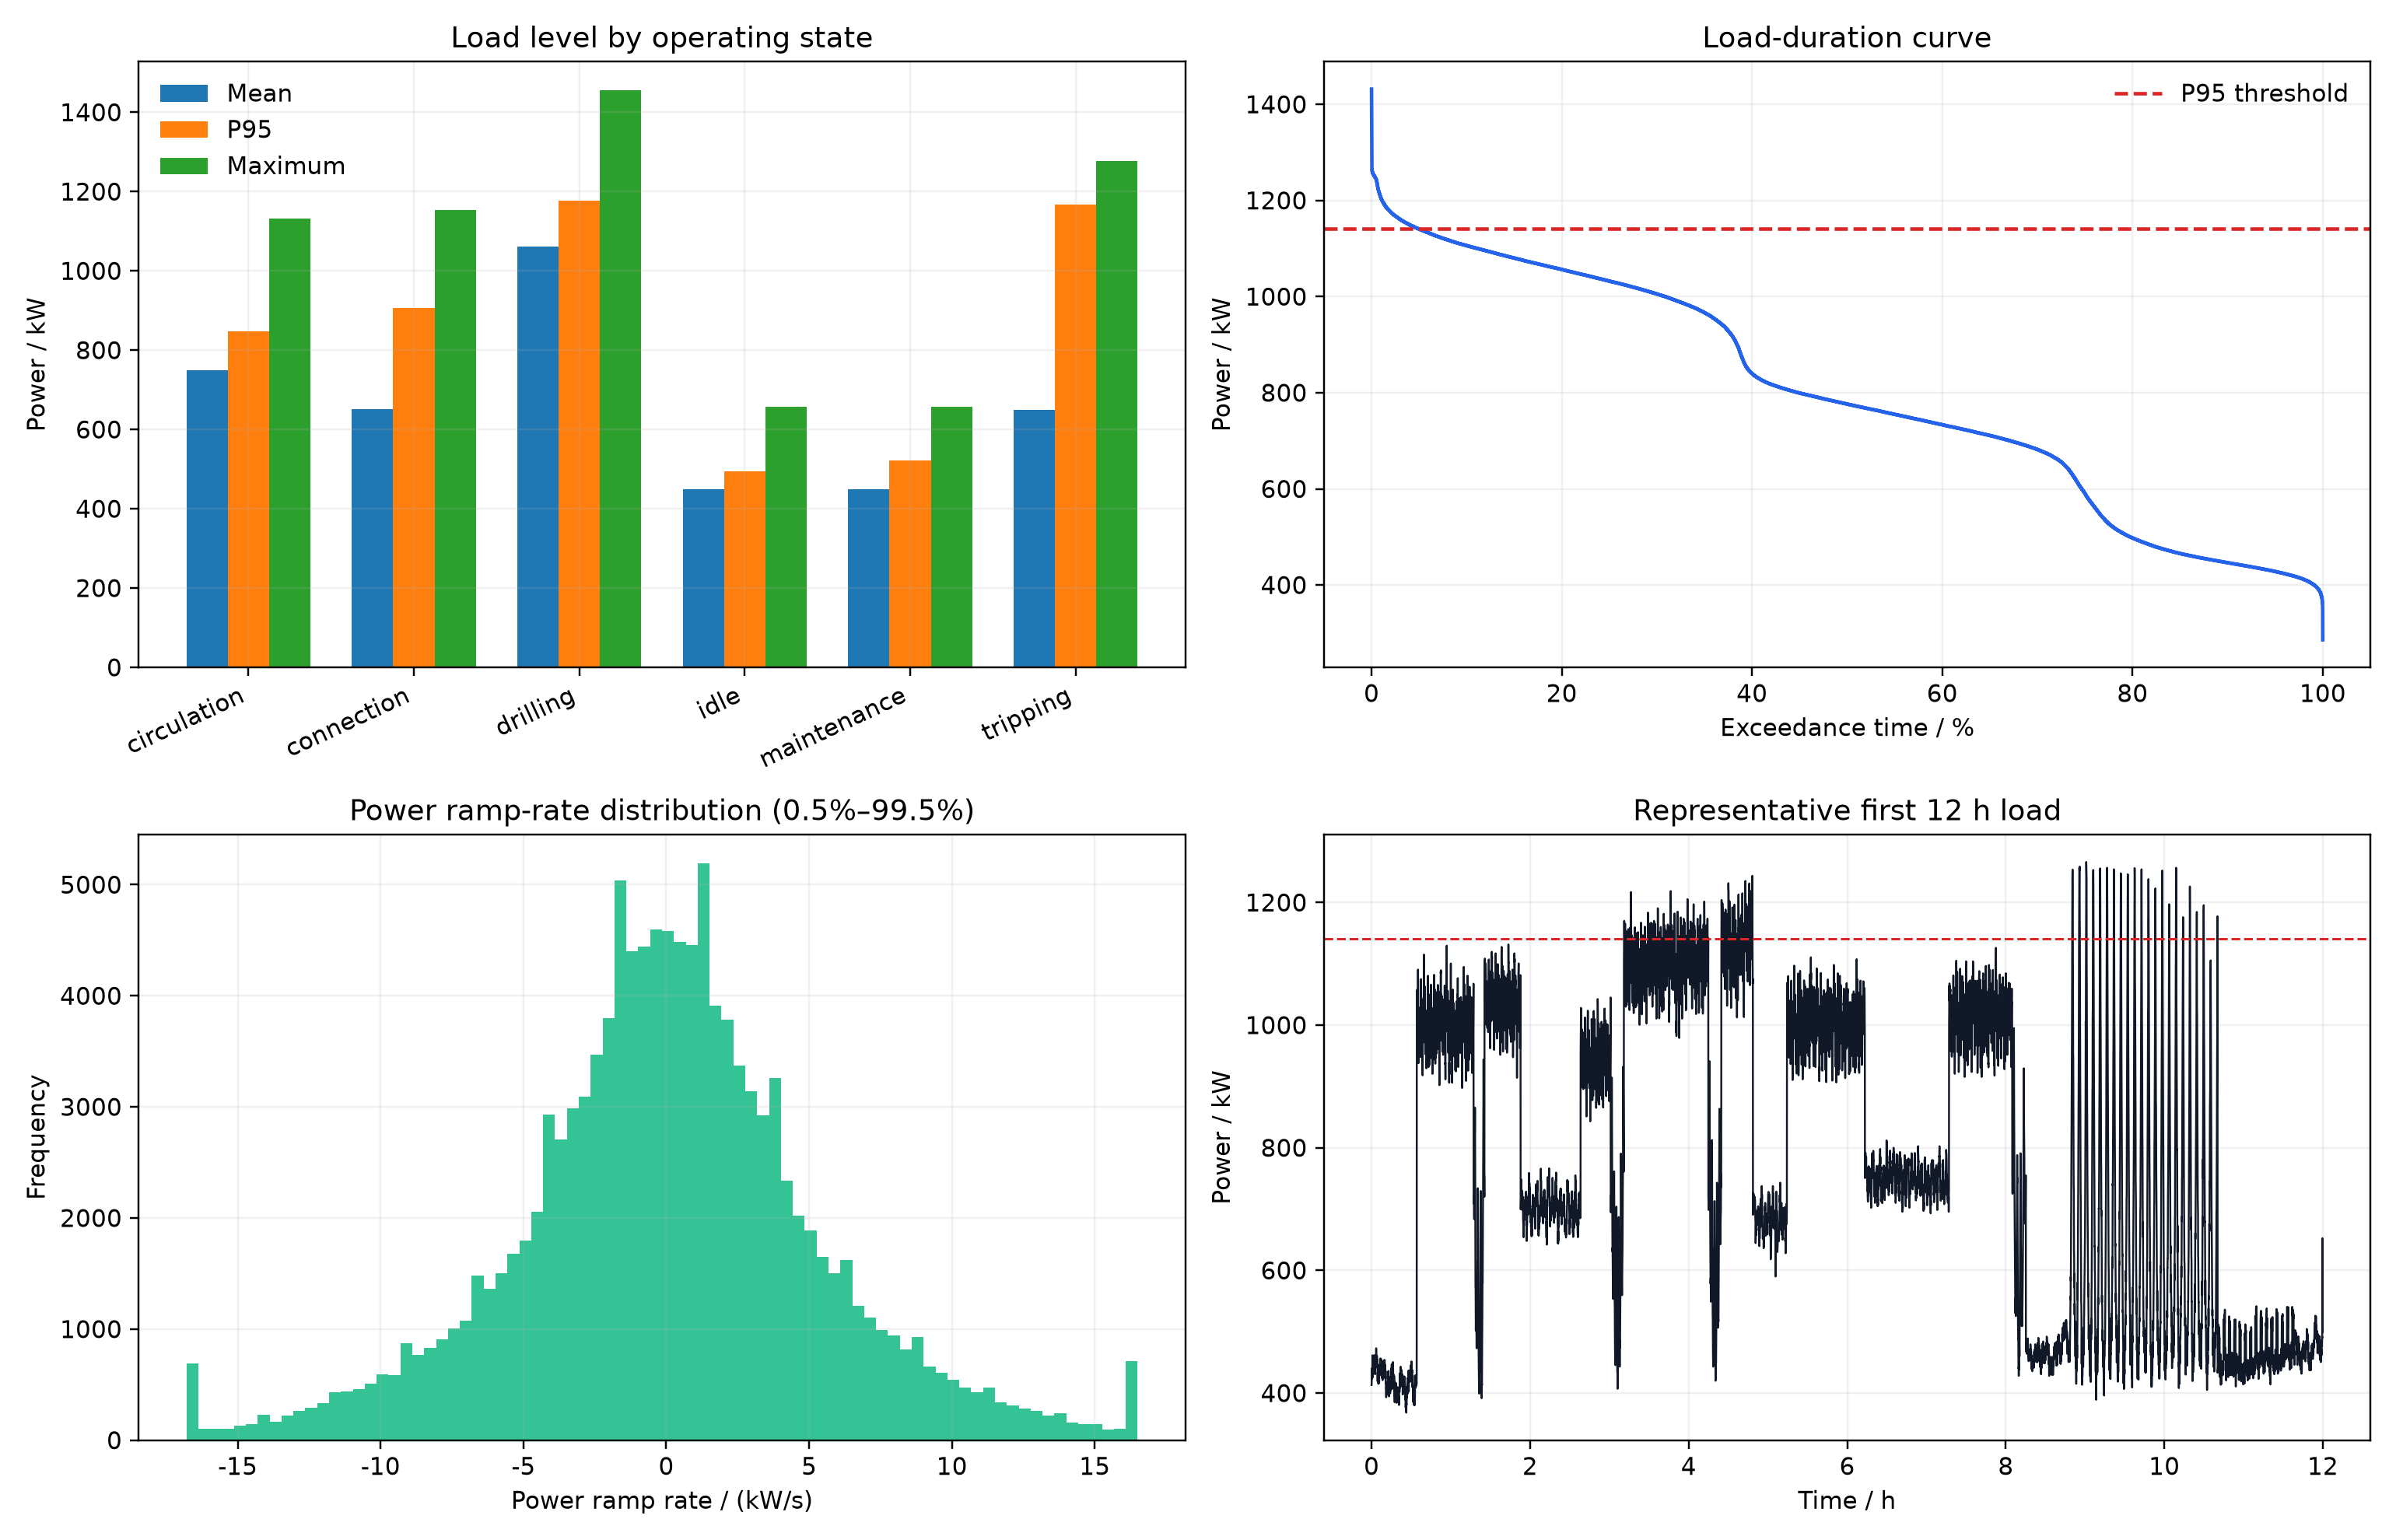
\includegraphics[width=\linewidth,keepaspectratio]{fig02_load_feature_summary_en.png}
\caption{Load-feature summary across operating states and representative
intervals}
\label{fig:load-summary}
\end{figure}

\begin{figure}
\centering
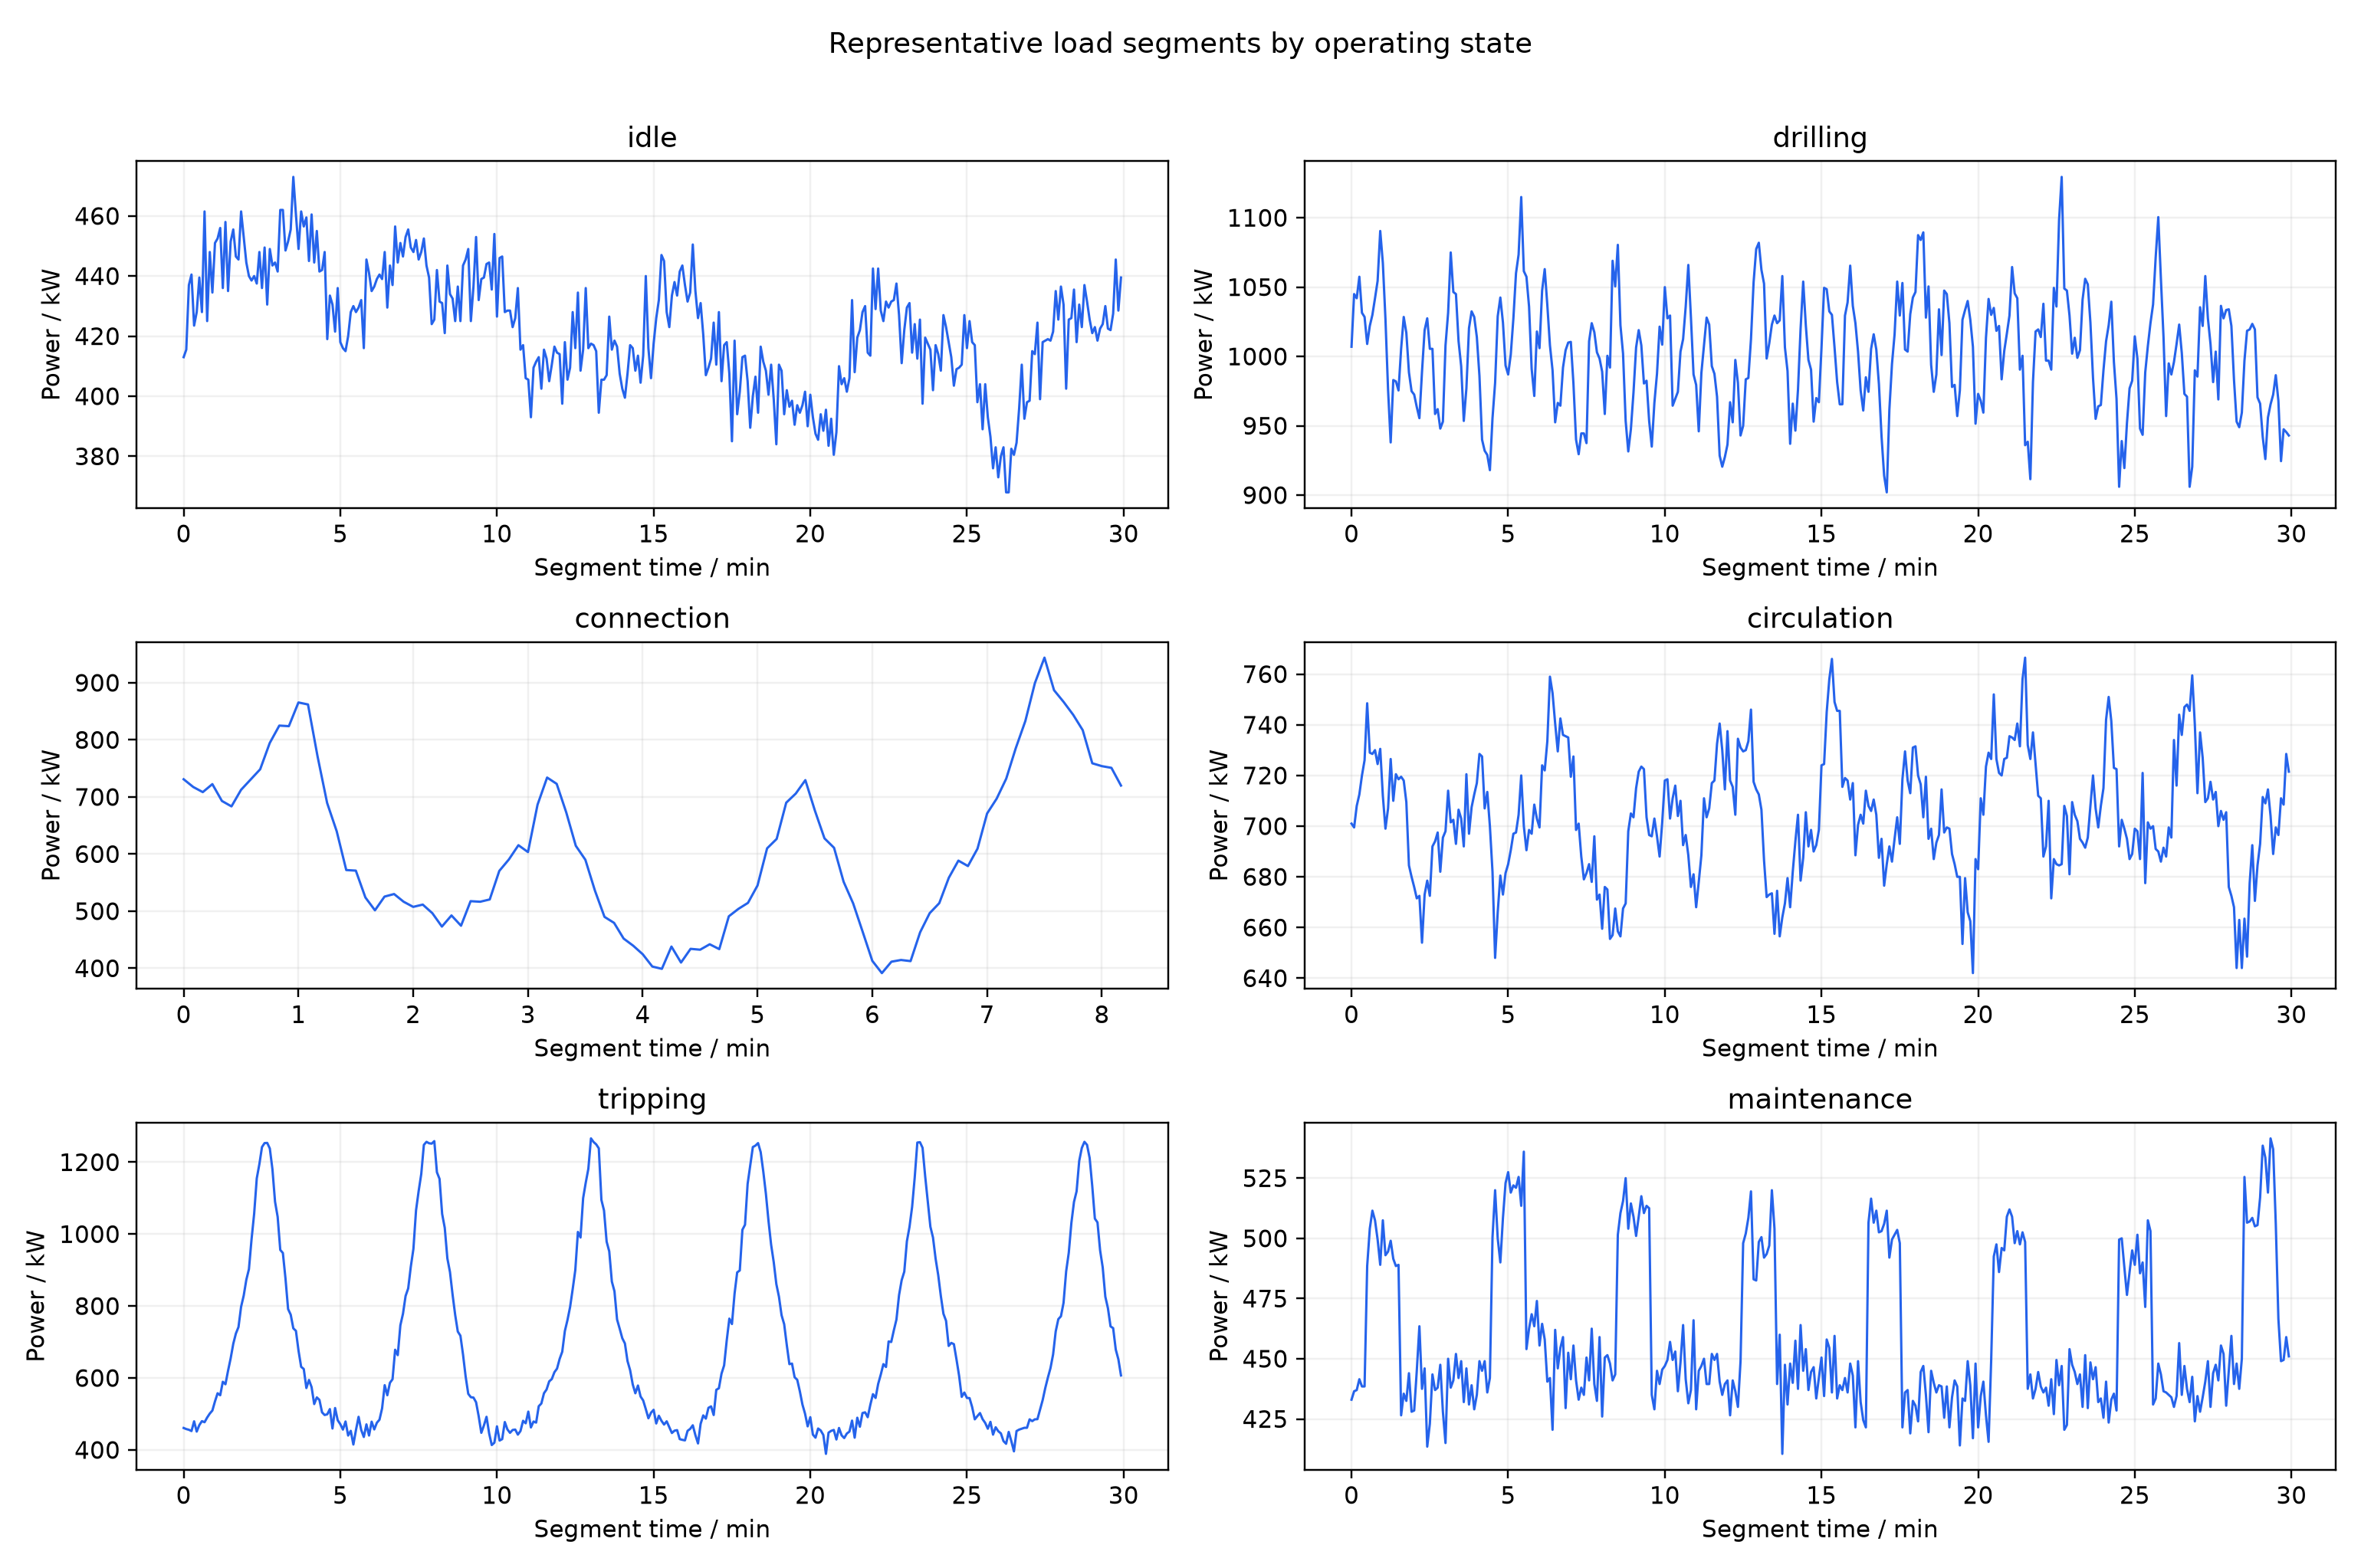
\includegraphics[width=\linewidth,keepaspectratio]{fig03_typical_state_curves_en.png}
\caption{Representative load curves for six drilling operating states}
\label{fig:state-curves}
\end{figure}

\begin{table}[!t]
\caption{Evaluation datasets and their roles}
\label{tab:datasets}
\centering
\footnotesize
\begin{tabular}{@{}
  >{\raggedright\arraybackslash}p{(\linewidth - 6\tabcolsep) * \real{0.21}}
  >{\raggedright\arraybackslash}p{(\linewidth - 6\tabcolsep) * \real{0.20}}
  >{\raggedleft\arraybackslash}p{(\linewidth - 6\tabcolsep) * \real{0.17}}
  >{\raggedright\arraybackslash}p{(\linewidth - 6\tabcolsep) * \real{0.42}}@{}}
\toprule
\begin{minipage}[b]{\linewidth}\raggedright
Dataset / source
\end{minipage} & \begin{minipage}[b]{\linewidth}\raggedright
Role
\end{minipage} & \begin{minipage}[b]{\linewidth}\raggedleft
Resolution
\end{minipage} & \begin{minipage}[b]{\linewidth}\raggedright
Content and provenance
\end{minipage} \\
\midrule
Development replay & Forecast selection, scenario calibration, and debugging &
5 s & One 72 h simulator seed; excluded from primary controller inference \\
Prospective simulator holdouts & Confirmatory dispatch comparison & 5 s & First
12 upstream-eligible 72 h seeds retained in frozen queue order \\
Energistics Well B; Utah FORGE 58-32 & Real drilling-process assumption audit &
1 min derived & 18,597 and 56,682 state-labeled minutes; no synchronized rig-bus
active power \\
REFIT houses 1--5 and 11; UCI household; Tsukuba & Confirmatory cross-domain
load forecasting & 1 min & Eight series from three dataset families; direct aggregate
power except the measurement-derived Tsukuba load target \\
M5BAT Pb1; Tsukuba & Observational BESS behavior audit & 1 min & Real power,
SOC, and available control/setpoint channels; not generated by RSS \\
OpenCEM; Petrobras 3W & Development/scope audit only & source-dependent & Opened
OpenCEM pilot excluded from confirmation; 3W anomaly labels not treated as
supply-risk labels \\
\bottomrule
\end{tabular}
\end{table}

\subsection{Preprocessing and
causality}\label{preprocessing-and-causality}

The preprocessing path canonicalizes timestamps, checks the sampling
interval, records quality flags, and imputes only the documented short
gaps. The forecast input window is constructed from information
available at the prediction timestamp. Transition features are based on
history, not on the future operation-state label. This distinction is
essential because a future-derived transition flag would make the
forecast or controller appear stronger while being unavailable during
online operation.

Development cases and holdout cases are separated throughout the evaluation.
Controller settings and eligibility criteria are fixed before prospective
holdout outcomes are inspected, and no parameter is retuned during the
12-holdout primary comparison.
Eligibility is determined before dispatch from the public-calibration audit,
operation-state codes, transition flags, and supply regime. The resulting
holdouts remain draws from the same mechanistic simulator and are not an
external-site dataset.

For the public electrical series, raw timestamps and units are normalized by
source-specific adapters, duplicate timestamps are rejected, and one-minute
records retain an explicit quality flag. The confirmatory forecast protocol
uses chronological 60/20/20 wall-clock partitions separated by one full UTC
day. Ridge regression and histogram gradient boosting are selected by
validation MAE and then refitted on training plus validation data. Persistence
and a 60-min rolling mean are fixed baselines. Mean absolute scaled error
(MASE), using adjacent quality-passing training minutes as the scale, is the
primary cross-dataset metric. The 1-min selected-model-versus-persistence
family is adjusted by Holm's method across eight series; 15- and 60-min results
are secondary and retain unadjusted day-cluster bootstrap intervals. The test
target for every listed series is opened once, and all dataset--horizon results
are retained regardless of direction.

The BESS analysis is observational. It tests AC/DC agreement, charge and
discharge efficiency, setpoint tracking where available, and whether the sign
of adjacent SOC change agrees with the power convention during active periods.
Eligible pairs are quality-passing adjacent one-minute records with
$|\Delta\mathrm{SOC}|\geq0.01$ percentage points and active-power magnitude of
at least 20~kW for M5BAT or 5~kW for Tsukuba. Directional consistency requires
$\operatorname{sign}(\Delta\mathrm{SOC})=-\operatorname{sign}(P)$ under the
adopted discharge-positive convention.
An initial M5BAT run produced no eligible rows because a released DC-power
field is numerically in kW despite its W suffix. That technically invalid run
is retained. The revised normalization was frozen only after annual raw-data
checks against current times voltage, and the corrected run is reported as R1.
The drilling-process analysis maps source-specific channels to coarse states,
aggregates the labels to one minute, and compares pooled contiguous state-run
durations with the simulator; it does not infer electrical power from
mechanical or hydraulic proxies. Unknown labels are retained as a state rather
than removed or bridged. In Energistics, 85.39\% of one-minute labels are
unknown, so its pooled dwell statistic is an assumption diagnostic rather than
a like-for-like state-conditional calibration target.

\section{Reserve--SOC supervisory coordination
framework}\label{reserve-soc-supervisory-coordination-framework}

\subsection{Forecasting module}\label{forecasting-module}

Let $L_t$ denote the total active load at time $t$, and let $H$ be the
forecast horizon. The forecasting module produces the point forecast in
Eq.~\eqref{eq:point-forecast}:

\begin{equation}
\label{eq:point-forecast}
\hat{\mathbf L}_{t+1:t+H}=f_\theta(\mathbf X_{t-W+1:t}),
\end{equation}

where $W$ is the historical input length and $\mathbf X$ contains the
available load, equipment, and causal process features. The comparison
includes Persistence, XGBoost, long short-term memory (LSTM), temporal
convolutional network (TCN), PatchTST, iTransformer, and state-aware ensemble
variants. The causal error-feedback ensemble supplies the point forecast used
by the controller under the frozen protocol. This path was fixed before the
prospective controller outcomes were generated; it was not selected by
inspecting their test errors. PatchTST and iTransformer provide established
transformer comparators \citep{nie2023patchtst,liu2024itransformer}.

For control, complete 12-step residual vectors are formed from the chronological
validation partition only. At each origin, 50 residual vectors are sampled by
strata of maximum positive forecast error and added to the causal point forecast:

\begin{equation}
\label{eq:forecast-scenarios}
\mathbf L^{(s)}_{t+1:t+H}=\max\{0,
\hat{\mathbf L}_{t+1:t+H}+\boldsymbol\epsilon^{(s)}_{1:H}\},
\end{equation}

where each residual block $\boldsymbol\epsilon^{(s)}_{1:H}$ is sampled as one
unit, preserving its within-horizon temporal dependence, and each scenario has
probability $1/50$. A chronological first-half/second-half audit within the
validation partition assesses interval and upper-tail coverage. Test targets
are neither read nor used to fit, rank, rescale, or select these scenarios.

\subsection{Supply, storage, and load
variables}\label{supply-storage-and-load-variables}

At each control step, the decision variables include grid power
$P^g_t$, generator power $P^{gen}_{i,t}$, unit commitment $u_{i,t}$,
storage charging power $P^{ch}_t$, storage discharging power $P^{dis}_t$,
and nonnegative unserved-load variables $U_t$. The BESS SOC is $S_t$,
and $\eta_{ch}$ and $\eta_{dis}$ denote charging and discharging
efficiencies. For a priority class $k$, $U_{k,t}$ is the load in that
class that is not served, so $0\leq U_{k,t}\leq L_{k,t}$ and
$U_t=\sum_k U_{k,t}$.

The physical balance for a scenario is represented by
Eq.~\eqref{eq:scenario-balance}:

\begin{equation}
\label{eq:scenario-balance}
L^{(s)}_t-U^{(s)}_t=P^{g,(s)}_t+\sum_i P^{gen,(s)}_{i,t}+P^{dis,(s)}_t-P^{ch,(s)}_t,
\end{equation}

where $U^{(s)}_t$ is nonnegative unserved load. This convention makes
the served load equal to $L^{(s)}_t-U^{(s)}_t$ and is also used when
computing unserved energy. The scenario-dependent storage state is updated by
Eq.~\eqref{eq:soc-dynamics}:

\begin{equation}
\label{eq:soc-dynamics}
S^{(s)}_{t+1}=S^{(s)}_t+\frac{\eta_{ch}P^{ch,(s)}_t\Delta t_h}{E_{BESS}}
-\frac{P^{dis,(s)}_t\Delta t_h}{\eta_{dis}E_{BESS}},
\end{equation}

where $\Delta t_h=5/3600$ h. All scenarios begin from the same measured SOC.
The model also enforces SOC bounds, charge/discharge exclusivity, and unit-
commitment constraints. The dispatch configuration uses a 5~s control interval,
a 30~min evaluation window with a 10~min warm-up, a 1300~kW grid limit,
four 240~kW generator units, a 500~kW/133~kWh BESS, initial SOC 0.65, SOC
bounds [0.15, 0.90], and charge/discharge efficiencies of 0.95. The unit
minimum stable output is 120~kW, the unit ramp limit is 30~kW per control
step, and the minimum up/down times are 12/6 steps. A start command reaches
synchronized minimum-stable output after six steps (30~s); the execution layer
prevents earlier generation. The V24 confirmatory analysis uses this fixed
30-s delay and does not include a startup-delay sweep. Available BESS power is
linearly derated within 5 percentage points of
the lower and upper SOC limits. The cost configuration
uses 0.71 yuan/kWh for grid energy, 7.50 yuan/L for
diesel, 0.15 yuan/kWh for storage degradation, 100 yuan/kWh for unserved
energy, and 5 yuan per start command. These values define a configured
operating-cost proxy rather than a site-calibrated life-cycle cost and should
be replaced with site measurements during deployment. The 500~kW/133~kWh
storage setting has a nominal power-to-energy ratio of 3.76~h$^{-1}$; it is a
stress-test configuration, not a value identified from a target-rig asset. The
optimizer uses the same public CAT XQP300 50-Hz piecewise fuel curve used to
report fuel consumption: 33.8, 47.3, and 62.5~L/h at 50\%, 75\%, and 100\%
load, respectively.\footnote{Caterpillar, \emph{XQP300 Mobile Generator Sets},
product specification, accessed 15 September 2026:
\url{https://www.cat.com/en_ID/products/new/power-systems/electric-power/mobile-generator-sets/1000024412.html}.}
The MILP includes the minimum-load fuel intercept and a second segment above
75\% unit load. Dispatch is
solved with HiGHS 1.12.0 through SciPy 1.17.1, using a 5~s time limit and a
$1.00\times10^{-4}$ relative MIP gap for every MILP path. The recorded decision latency covers
forecast-to-dispatch computation.

For each generator unit, the MILP enforces the minimum-stable and rated-power
bounds, the ramp limits, and the logical relation between commitment,
startup, and shutdown variables. Minimum up/down constraints include the
executed transition history at the beginning of each horizon. The first
control action is shared across forecast scenarios, whereas later
continuous recourse variables may differ by scenario. This prevents the
controller from using future scenario identity to choose the first physical
action.

\subsection{Dispatch objective}\label{dispatch-objective}

The receding-horizon controller minimizes expected operating cost plus a
CVaR penalty on shortage cost over the current horizon, as defined in
Eq.~\eqref{eq:dispatch-objective}:

\begin{equation}
\label{eq:dispatch-objective}
\begin{aligned}
\min J &= \mathbb E_s\left[J_{energy}^{(s)}+J_{fuel}^{(s)}+J_{start}^{(s)}+J_{deg}^{(s)}\right.\\
&\quad\left.+J_{short}^{(s)}+J_{spill}^{(s)}\right]
+\beta\operatorname{CVaR}_{\alpha}\left(J_{short}^{(s)}\right).
\end{aligned}
\end{equation}

Here $J_{short}^{(s)}$ is the shortage penalty for scenario $s$,
$J_{spill}^{(s)}$ penalizes unused surplus, and the scenario probability is
$1/S$. The CVaR term is implemented with an auxiliary threshold $\eta$ and
excess variables $\xi_s$ in Eq.~\eqref{eq:cvar-linearization}:

\begin{equation}
\label{eq:cvar-linearization}
\operatorname{CVaR}_{\alpha}(J_{short})=\eta+\frac{1}{(1-\alpha)S}\sum_{s=1}^{S}\xi_s,
\qquad \xi_s\geq J_{short}^{(s)}-\eta,\quad \xi_s\geq0.
\end{equation}

This auxiliary-variable representation is the standard linearizable CVaR
construction \citep{rockafellar2000cvar}; the stochastic-MILP and robust
cost--risk literature provides related scheduling precedents
\citep{franke2020stochasticmilp,ji2018robustcvar}.

The scenario set contains 50 equally weighted validation-residual trajectories.
The primary CVaR setting is $(\alpha,\beta)=(0.90,1.00)$; for risk levels 0,
1, 2, and 3, respectively, $\alpha$ is 0.80, 0.85, 0.90, and 0.90, while
$\beta$ is 1.00, 1.00, 1.50, and 2.00. Thus, the smallest represented tail
contains five equally weighted scenarios. A pre-run discretization gate rejects
any setting with fewer than five effective tail scenarios. The more expensive
$S=100$, $\alpha=0.95$ setting is reserved for offline sensitivity because
development solves approached or exceeded the 5~s control interval.
The commitment variables are integer and include generator availability,
minimum stable output, ramping, minimum up/down time, and startup/shutdown
logic. Every MILP comparison uses the same realized replay, plant, prices,
initial state and pending start history, risk-conditioned terminal-SOC rule,
horizon, solver backend, time limit, and MIP gap. Predicted horizon CVaR is
reported separately from realized accounting. Realized operating cost contains
grid energy, diesel fuel, storage throughput, and start commands;
terminal-energy adjustment and VOLL times EENS are separate columns. Their sum
is called total social cost, not risk-adjusted operating cost.

\subsection{Reserve--SOC supervisory layer}\label{soc-supervisory-layer}

The supervisory layer selects the operating mode around the rolling dispatch
controller while retaining the constraints of the physical model. It uses
current SOC, available capacity, the causal risk signal, and the forecasted
supply--demand envelope. In normal operation, the controller uses
risk-adaptive CVaR MPC; under protection, it uses a deterministic
reserve-envelope MPC (implementation label \texttt{ML-Robust-MPC}). This path
does not solve a min--max or uncertainty-set robust-optimization problem: it
adds a fixed 10~kW reserve and a disagreement envelope equal to 0.25 times the
absolute point-forecast--persistence difference. Protection begins when the
risk level is at least 2 or SOC is at most 0.30. Normal operation
resumes when the risk level is at most 1, SOC is at least 0.35, and both
conditions persist for 12 control steps.

When protection is active and SOC is at most 0.30, the controller requests at
least two model-reachable generator units if the forecast-deficit guard is
triggered. A grid-headroom rule targets SOC 0.75 and limits the storage
adjustment to 20\% of rated storage power. This rule preserves reserve without
starting an additional generator solely to charge the battery.

The causal four-level risk target is formed from the realized future peak only
for offline labeling. A safety margin of $\max(50~\mathrm{kW},,0.05L_{peak})$
is subtracted from available supply, and the resulting margin ratio defines
normal, watch, warning, and severe classes at thresholds 0.15, 0.05, and 0.
The online classifier receives only current and historical features; future
load and future-derived state indicators are excluded. These thresholds and
the supervisor thresholds above were frozen before V24 and were not subjected
to a confirmatory threshold sweep.

\subsection{Auxiliary risk interface}\label{auxiliary-risk-interface}

Earlier development also tested evidence-fusion variants of the four-level risk
signal. They changed recognition and probability diagnostics but did not improve
energy outcomes under the matched replay. Those negative results and their full
definitions are retained in the supplementary reproducibility record; evidence
fusion is not part of the V24 method or primary claim.

\subsection{Emergency load
protection}\label{emergency-load-protection}

When total available supply cannot satisfy all loads, the emergency
module allocates supply by priority. Critical loads are protected first,
essential loads are protected second, and interruptible loads absorb the
remaining deficit. The controller reports both critical load unserved
energy and total unserved energy. A reduction in critical load shortage
does not imply that total shortage has been eliminated.

Table~\ref{tab:symbols} summarizes the principal symbols and configured
constraints.

\begin{table}[!t]
\caption{Symbols and constraints}
\label{tab:symbols}
\centering
\footnotesize
\begin{tabular}{@{}
  >{\raggedright\arraybackslash}p{(\linewidth - 6\tabcolsep) * \real{0.2308}}
  >{\raggedright\arraybackslash}p{(\linewidth - 6\tabcolsep) * \real{0.2308}}
  >{\raggedleft\arraybackslash}p{(\linewidth - 6\tabcolsep) * \real{0.3077}}
  >{\raggedright\arraybackslash}p{(\linewidth - 6\tabcolsep) * \real{0.2308}}@{}}
\toprule
\begin{minipage}[b]{\linewidth}\raggedright
Symbol / group
\end{minipage} & \begin{minipage}[b]{\linewidth}\raggedright
Meaning
\end{minipage} & \begin{minipage}[b]{\linewidth}\raggedleft
Unit
\end{minipage} & \begin{minipage}[b]{\linewidth}\raggedright
Parameter provenance / configuration
\end{minipage} \\
\midrule
$L_t$ & total rig active load & kW & mechanistic evaluation record \\
$P^g_t$ & grid active power & kW & 1300 kW grid limit \\
$P^{gen}_{i,t}$ & generator $i$ active power & kW & four 240 kW units \\
$u_{i,t}$ & generator commitment & binary & MILP formulation \\
$P^{ch}_t$, $P^{dis}_t$ & BESS charging and discharging power & kW & 500 kW BESS limit \\
$S_t$ & BESS state of charge & \% or p.u. & initial 0.65; bounds [0.15, 0.90] \\
$U_t$ & nonnegative unserved load; sum of class-level curtailed load & kW & priority-based allocation setting \\
$\Delta t_h$, $H$, $W$ & time step, forecast horizon, history length & h/steps & $5/3600$ h; 12-step horizon; 120-step history \\
$\beta$, $\alpha$ & CVaR weight and confidence level & --- & $\beta=1.00$ and $\alpha=0.90$ at base risk; risk-level settings stated in Section~4.3 \\
\bottomrule
\end{tabular}
\end{table}

\section{Experimental protocol}\label{experimental-protocol}

\subsection{Research questions}\label{research-questions}

The experiments address four questions:

\textbf{RQ1.} How do the forecasting candidates compare on total-load,
peak, and transition errors under the same replay?

\textbf{RQ2.} Does reserve--SOC supervision reduce EENS, and how much
additional realized operating cost does it require relative to rule-based
control and matched point-forecast and residual-CVaR MILPs?

\textbf{RQ3.} Which control components change the physical dispatch, and does
the controller remain feasible under generator, grid, storage, missing-data,
and telemetry disturbances?

\textbf{RQ4.} Which parts of the evidence chain transfer to public real
measurements, and which simulator assumptions are challenged by external
checking?

RQ3 is examined through leave-one-component-out interventions for residual
scenarios, adaptive CVaR, SOC supervision, and generator-first execution,
together with retained disturbance diagnostics and model-constraint audits.
The confirmatory V24 evidence does not contain a startup-delay, economic-weight,
or supervisor-threshold sweep. RQ4 is examined through frozen multi-horizon load
forecasting, observational BESS power--SOC checks, and state-dwell comparison
against two independent drilling-process records. None of the RQ4 analyses is
treated as a causal closed-loop test of RSS.

\subsection{Baselines}\label{baselines}

The forecasting baselines are Persistence, XGBoost, LSTM, TCN, PatchTST,
iTransformer, and state-aware or ensemble variants. This set includes a
naive reference, classical machine learning, recurrent neural networks,
convolutional sequence modeling, and recent transformer-based models.
For compact tables, the longer forecasting labels are abbreviated as follows:
state-aware patch transformer (SA-PT), causal error-feedback ensemble (CEF),
validation-weighted ensemble (VWE), state-aware dual-branch patch transformer
(SA-DB), and state-aware TCN-attention (SA-TA).

The primary dispatch paths are rule-based control (RB), persistence MILP,
matched point-forecast MILP, fixed-reserve MILP, residual-CVaR MILP,
risk-adaptive residual-CVaR MILP, and the full risk--SOC supervisory MILP
(RSS). All MILP names describe one implementation path whose inputs or
supervisory switches are changed explicitly. RB is retained as a transparent
operational reference. Auxiliary evidence-fusion and perfect-foresight studies
from earlier development are not pooled with this primary comparison.
The three prespecified confirmatory references span distinct questions: RB is
the transparent operational comparator, point-forecast MILP is the matched
deterministic optimization comparator, and risk-adaptive residual-CVaR is the
immediate parent controller without the reserve--SOC supervisory layer. The
remaining paths characterize the implementation progression and component
mechanisms rather than enlarging the primary hypothesis family.

All online MILPs use the same plant model, realized load and availability,
initial SOC and unit history, price terms, terminal-SOC policy, solver, and
constraint-audit path. Persistence versus point forecast changes only the
forecast source; fixed reserve adds only the declared reserve; residual-CVaR
adds validation-calibrated scenarios and CVaR; risk adaptation changes only the
risk-conditioned CVaR coefficients; and RSS adds the supervisory state machine
and generator-first reserve action. Additional leave-one-out paths remove one
of these components from RSS.

\subsection{Metrics}\label{metrics}

Forecast metrics include mean absolute error (MAE), root mean squared
error (RMSE), the coefficient of determination ($R^2$), normalized MAE,
sMAPE, peak MAE, and transition MAE. Transition MAE is reported because
average error can hide the short events that determine generator
commitment and storage reserve.

Dispatch metrics include total and normalized EENS, loss-of-load duration,
realized operating cost, terminal-energy adjustment, reliability penalty,
total social cost, predicted horizon CVaR, diesel fuel, start commands and
synchronizations, minimum SOC, maximum decision latency, and constraint-audit
failures. Risk-interface
metrics include Macro-F1, balanced accuracy, high- and severe-risk recall,
multiclass Brier score, mean ignorance, mean conflict, changed risk levels, and
changed physical actions.
Constraint audits check active-power balance, dynamic grid/generator/storage
capacity, SOC bounds, simultaneous charge/discharge, integer commitment,
startup synchronization delay, and solver/runtime validity.

EENS is the sole primary endpoint. Realized operating cost is the principal
economic secondary endpoint and excludes both EENS monetization and predicted
CVaR. Terminal-energy adjustment and VOLL times EENS are reported separately,
so a reliability improvement cannot be restated as an independent cost benefit
created by the same penalty.

\subsection{Reproducibility protocol}\label{reproducibility-protocol}

Development and holdout cases are separated before controller comparison. The
primary analysis uses the first 12 eligible seeds from the prospectively
declared queue and treats the seed as the independent unit, with three
30-min scored operating scenarios clustered within each seed after separate
10-min warm-ups. Thus each seed contributes 1.5 scored hours. Exact
two-sided sign-flip tests, 20,000-resample seed bootstrap intervals, and Holm
correction across the three primary controller contrasts are applied at seed
level.
Upstream eligibility is evaluated before controller execution from the
public-calibration audit, operation-state codes, transition flags, and supply
regime. Seed processing follows the declared queue order; no outcome-based
replacement is permitted.

Previously inspected seeds are development-only. The prospective queue is
processed in order; eligibility is written before dispatch and is based only on
operation-state and supply-regime coverage. Every eligible result is retained
regardless of direction, including null, adverse, failed, and timed-out cases.
Versioned configurations, ordered seed lists, hashes, and trajectory-level
audit results are retained in the working evidence ledger and are required in
the updated reproducibility package.

Earlier aborted protocol artifacts remain read-only and are not pooled with the
confirmatory analysis. V24 uses a wholly unseen queue (20261120 onward), a
full-seed serial-execution lock, explicit failure records, and a 5-s wall-clock
gate. If no learned risk candidate passes the prespecified validation gates, an
always-severe dispatch-facing fallback is applied without excluding the seed;
fallback use is reported and is not described as learned-risk certification.

Table~\ref{tab:protocol} distinguishes the forecasting and dispatch protocols.

\begin{table}[!t]
\caption{Experimental comparison protocol}
\label{tab:protocol}
\centering
\footnotesize
\begin{tabular}{@{}
  >{\raggedright\arraybackslash}p{(\linewidth - 4\tabcolsep) * \real{0.3333}}
  >{\raggedright\arraybackslash}p{(\linewidth - 4\tabcolsep) * \real{0.3333}}
  >{\raggedright\arraybackslash}p{(\linewidth - 4\tabcolsep) * \real{0.3333}}@{}}
\toprule
\begin{minipage}[b]{\linewidth}\raggedright
Item
\end{minipage} & \begin{minipage}[b]{\linewidth}\raggedright
Forecast comparison
\end{minipage} & \begin{minipage}[b]{\linewidth}\raggedright
Dispatch comparison
\end{minipage} \\
\midrule
Evaluation basis & Simulated development replay plus eight frozen public real
electrical series & Power-system simulation \\
Sampling & 5 s for development; 1 min for public real data & 5 s control/evaluation path \\
Forecast window & 10 min history $\rightarrow$ 1 min in development; causal
lags and 1/15/60-min horizons in public data & same forecast package per dispatch
comparison \\
Baselines & 11 development candidates; persistence and 60-min rolling mean for
public confirmation & RB plus six matched MILP
paths; four leave-one-component-out interventions are exploratory \\
Main split & fixed development boundaries; public series use chronological
60/20/20 wall-clock partitions with one-day gaps & first 12 eligible prospective
holdouts; three scenarios clustered per seed \\
Primary metrics & development MAE; public-data MASE with MAE/RMSE companions & EENS \\
Additional checks & peak/transition error, day-cluster intervals, runtime & operating cost, loss-of-load duration,
SOC, fixed-delay synchronization, latency, and constraint audit \\
Reproducibility & fixed splits, test-open-once rule, data/config hashes, and
software environment & fixed controller settings, seed queue, hashes, seed-level
statistics, and constraint audits \\
\bottomrule
\end{tabular}
\end{table}

The forecast models use 120 historical steps (10~min) to predict 12 steps
(1~min), batch size 512, a maximum of 20 training epochs, early-stopping
patience of 5, learning rate $8.00\times10^{-4}$, weight decay
$1.00\times10^{-4}$, and seed
20260902. The replay was run with Python 3.11.16, PyTorch 2.9.1, XGBoost
3.2.0, and an NVIDIA GeForce RTX 5060 Laptop GPU.

\section{Results}\label{results}

\subsection{Forecasting comparison}\label{forecasting-comparison}

Table~\ref{tab:forecast-results} summarizes the prespecified development
replay. The validation-weighted ensemble (VWE) obtains the lowest MAE
(19.63~kW), while the causal error-feedback ensemble (CEF) used by the
controller obtains 20.25~kW, 63.10\% below Persistence. VWE also has the
lowest RMSE (41.81~kW) and highest $R^2$ (0.972); CEF has the lowest peak MAE
(21.53~kW). These are development-replay comparisons, not independent field
validation and not a basis for changing the frozen prospective controller.

The forecasting comparison serves two purposes. It compares modern sequence
models and quantifies the validation residuals used by the dispatch controller,
and it
quantifies peak and transition errors that affect generator commitment and
storage reserve. CEF supplies the causal point forecast, while complete CEF
validation-residual vectors supply the uncertainty scenarios. The strongest
forecast is an existing iTransformer baseline; the contribution evaluated below
is the propagation of calibrated forecast uncertainty into the energy-management
decision.

Figure~\ref{fig:forecast-traces} separates overall behavior from a principal
target transition and shows four representative predictors: VWE (lowest MAE),
CEF (the controller's causal point forecast), PatchTST (a transformer
comparator), and Persistence (the naive reference).
Figure~\ref{fig:forecast-metrics} reports all candidates using the
abbreviations defined in Section~\ref{baselines}.

\begin{figure}
\centering
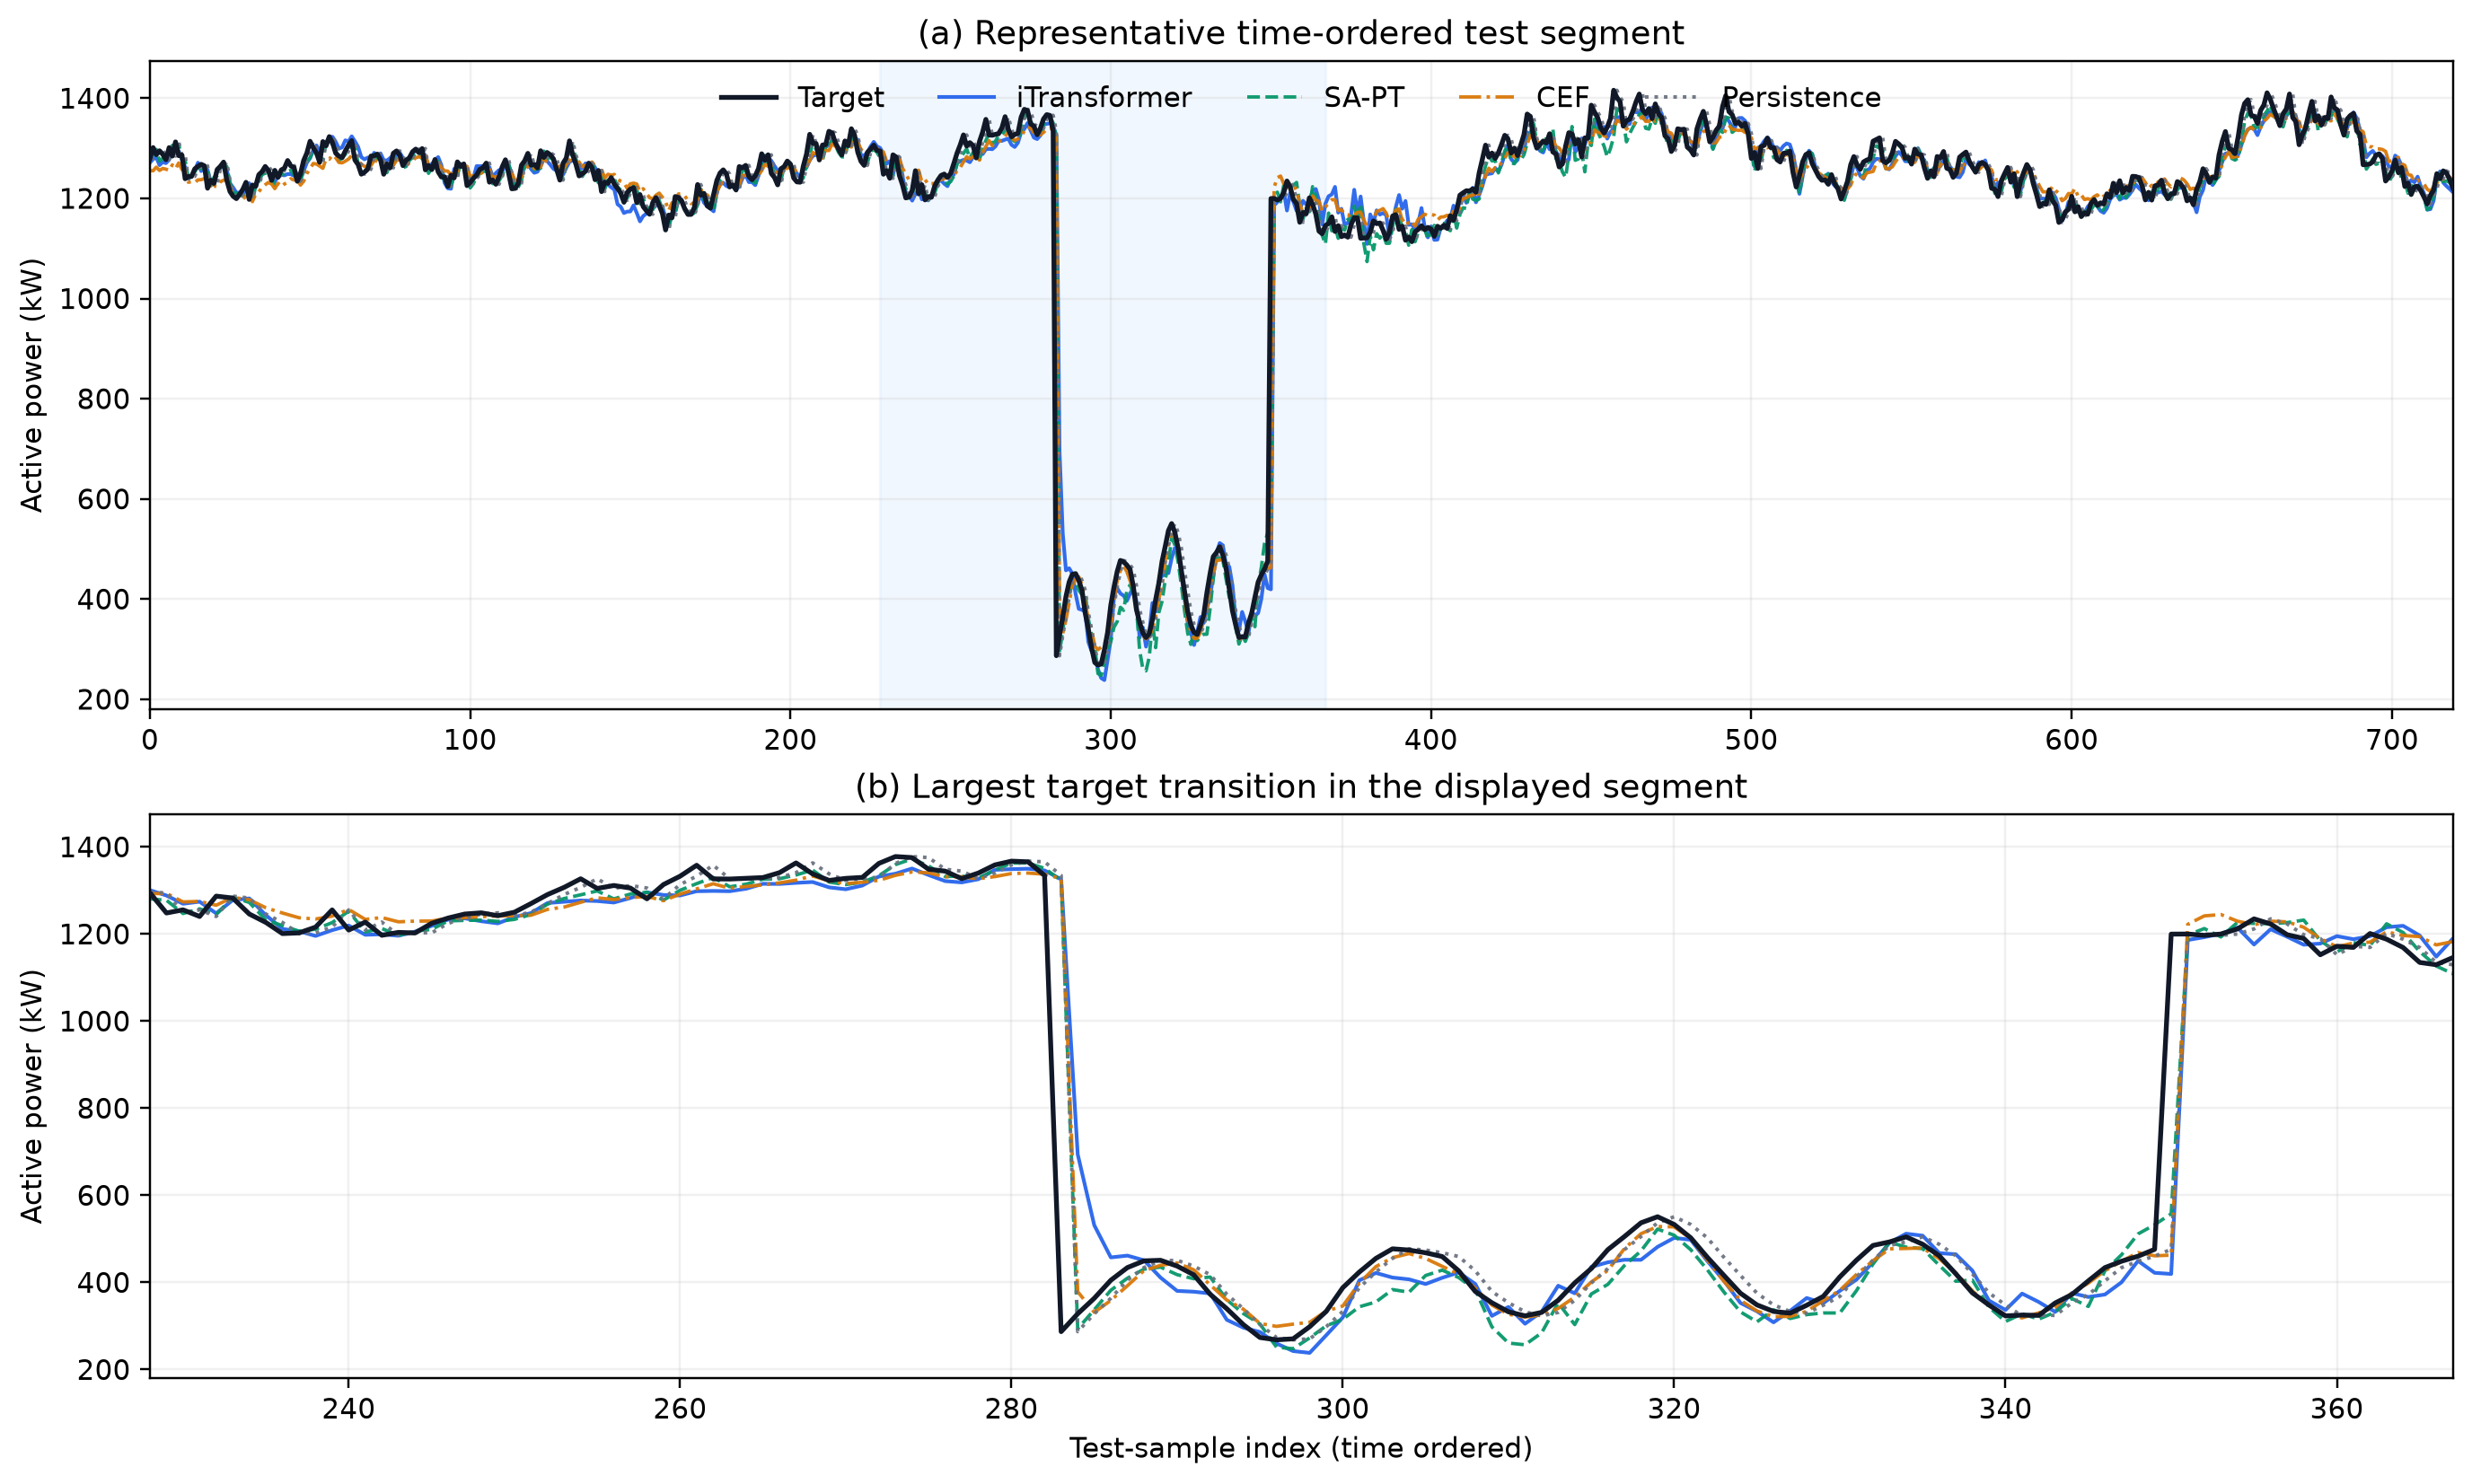
\includegraphics[width=\linewidth,keepaspectratio]{fig04_target_domain_forecast_traces_en.png}
\caption{Representative forecast traces and transition detail}
\label{fig:forecast-traces}
\end{figure}

\begin{figure}
\centering
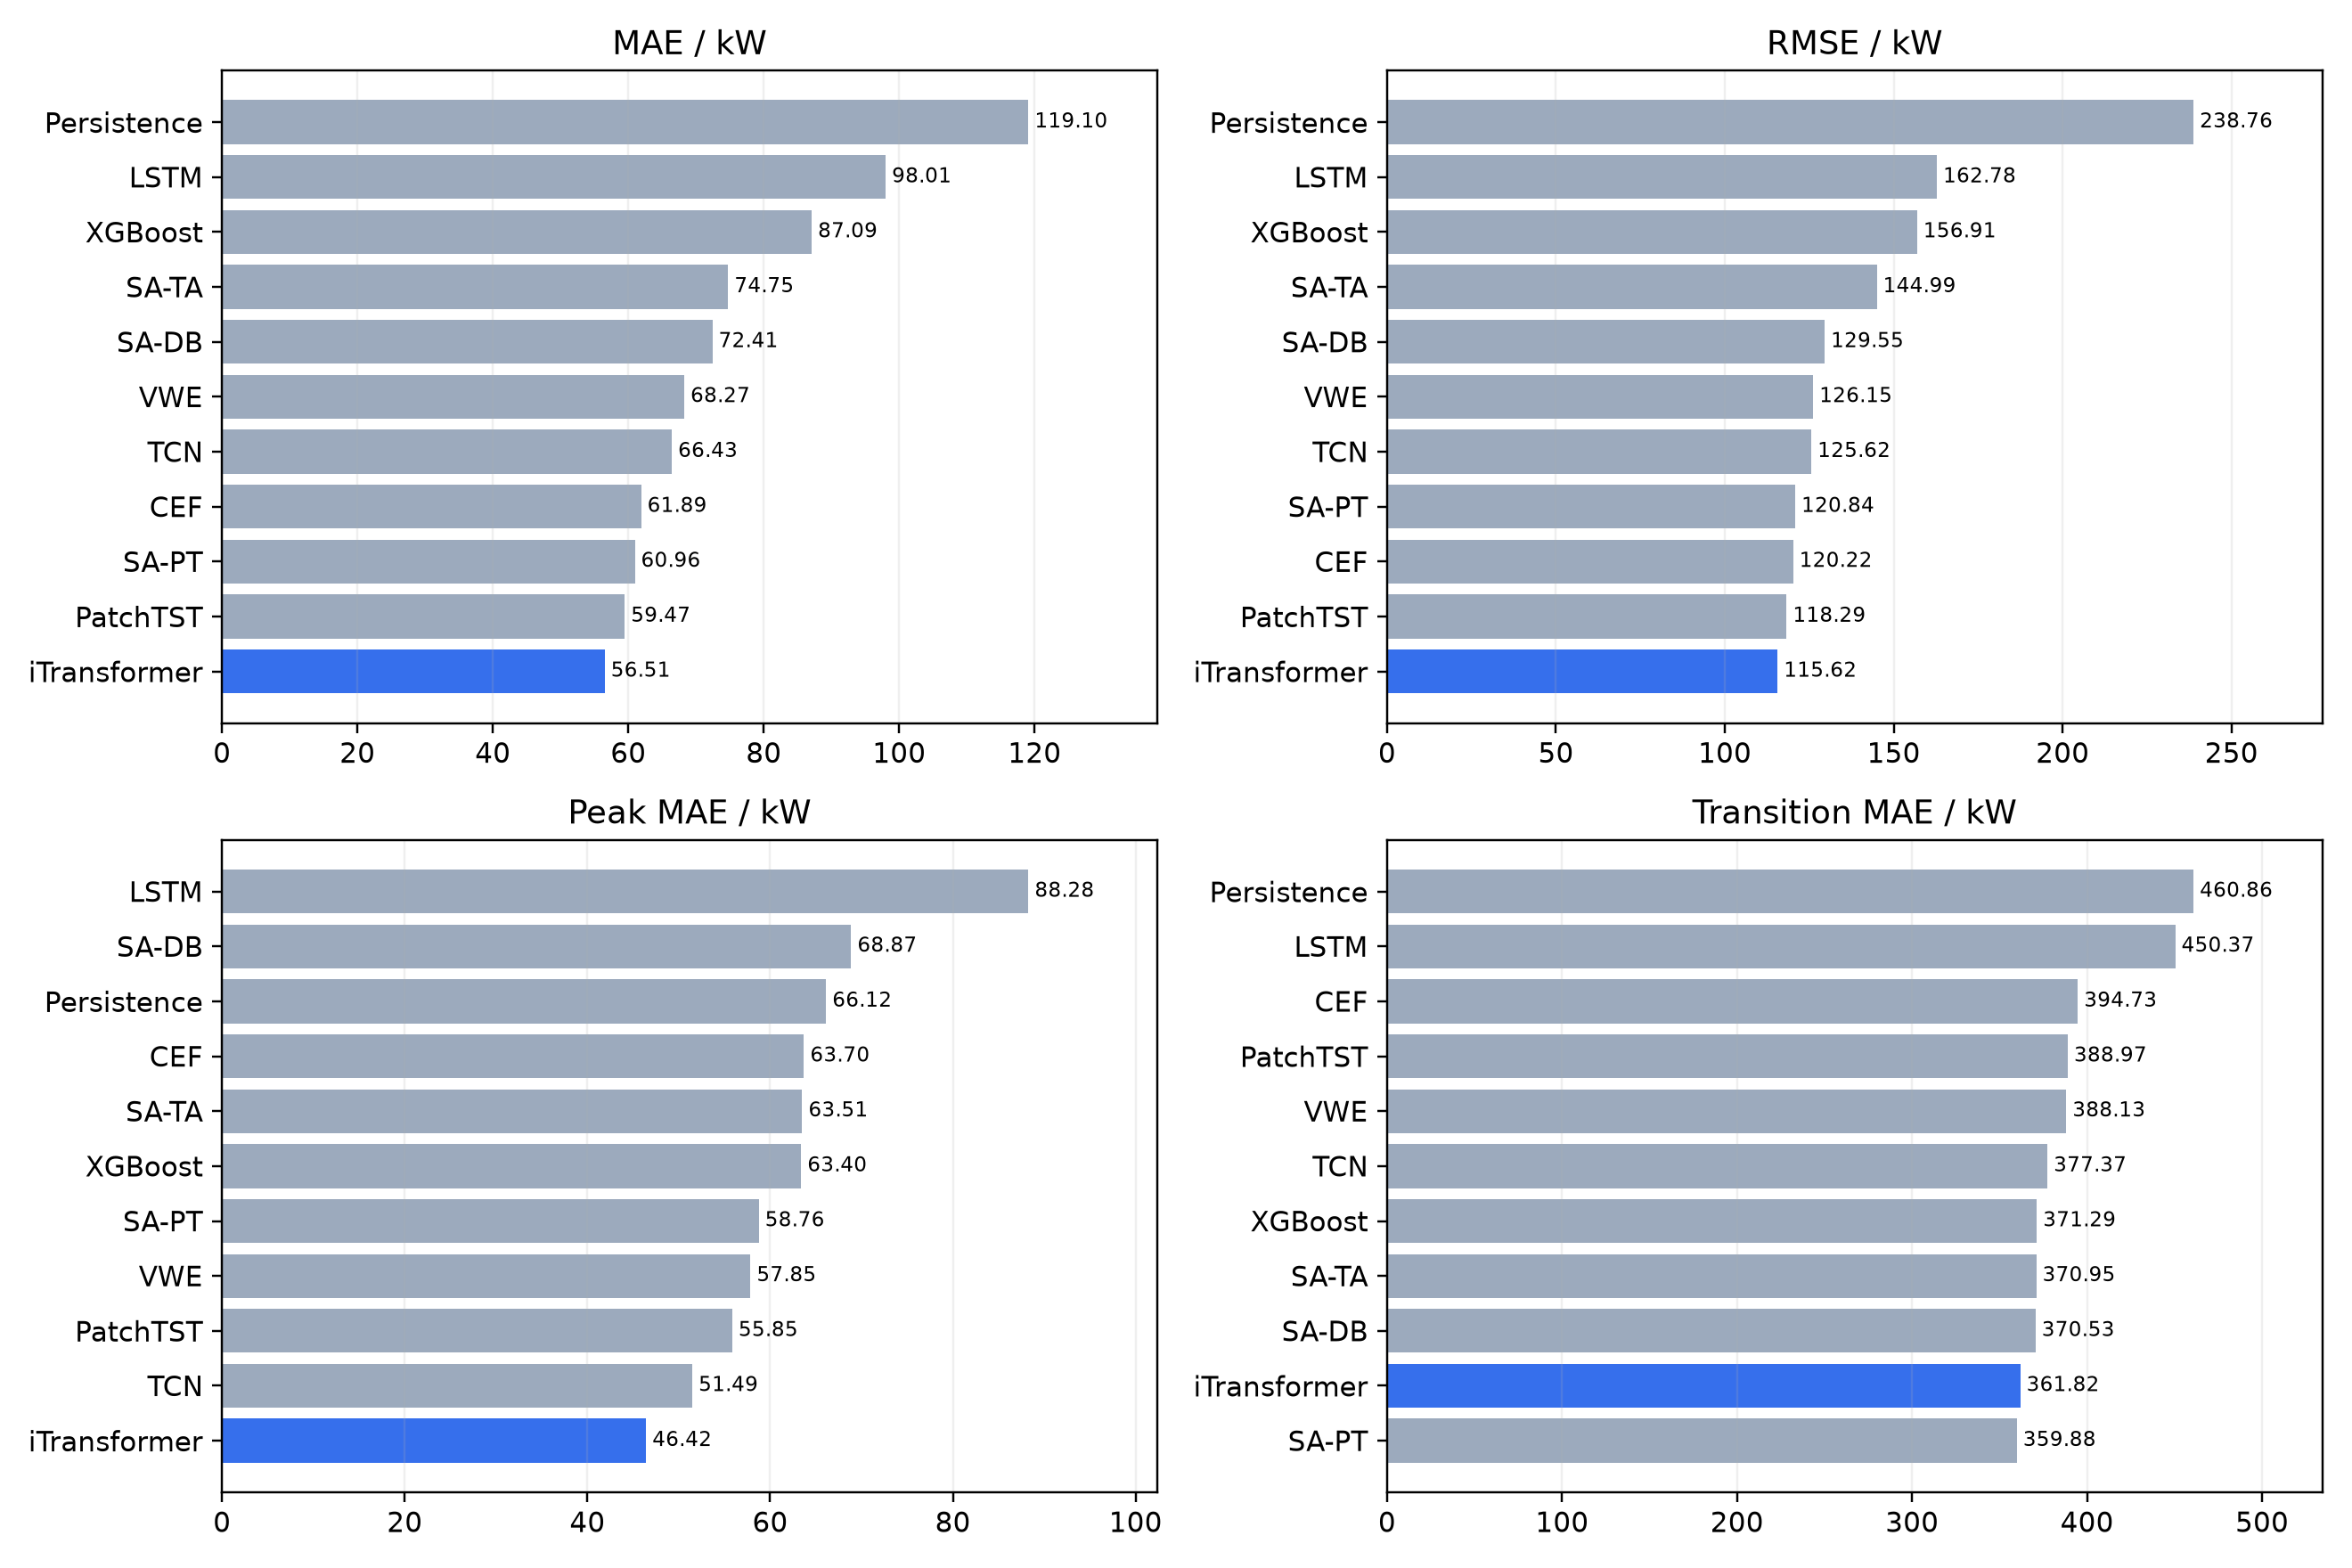
\includegraphics[width=\linewidth,keepaspectratio]{fig05_target_domain_forecast_metrics_en.png}
\caption{Forecast metric comparison for all candidates}
\label{fig:forecast-metrics}
\end{figure}

\begin{table}[!t]
\caption{Forecasting comparison on the evaluation replay}
\label{tab:forecast-results}
\centering
\footnotesize
\begin{tabular}{@{}
  >{\raggedright\arraybackslash}p{(\linewidth - 10\tabcolsep) * \real{0.2000}}
  >{\raggedleft\arraybackslash}p{(\linewidth - 10\tabcolsep) * \real{0.1600}}
  >{\raggedleft\arraybackslash}p{(\linewidth - 10\tabcolsep) * \real{0.1600}}
  >{\raggedleft\arraybackslash}p{(\linewidth - 10\tabcolsep) * \real{0.1600}}
  >{\raggedleft\arraybackslash}p{(\linewidth - 10\tabcolsep) * \real{0.1600}}
  >{\raggedleft\arraybackslash}p{(\linewidth - 10\tabcolsep) * \real{0.1600}}@{}}
\toprule
\begin{minipage}[b]{\linewidth}\raggedright
Model
\end{minipage} & \begin{minipage}[b]{\linewidth}\raggedleft
MAE (kW)
\end{minipage} & \begin{minipage}[b]{\linewidth}\raggedleft
RMSE (kW)
\end{minipage} & \begin{minipage}[b]{\linewidth}\raggedleft
$R^2$
\end{minipage} & \begin{minipage}[b]{\linewidth}\raggedleft
Peak MAE (kW)
\end{minipage} & \begin{minipage}[b]{\linewidth}\raggedleft
Transition MAE (kW)
\end{minipage} \\
\midrule
VWE & 19.63 & 41.81 & 0.972 & 22.37 & 156.17 \\
CEF & 20.25 & 42.81 & 0.971 & 21.53 & 158.70 \\
SA-TA & 21.16 & 43.00 & 0.970 & 23.20 & 156.38 \\
SA-DB & 21.27 & 43.51 & 0.970 & 23.92 & 158.17 \\
SA-PT & 21.64 & 44.14 & 0.969 & 23.21 & 158.15 \\
PatchTST & 22.84 & 47.11 & 0.964 & 23.55 & 165.39 \\
iTransformer & 22.84 & 47.68 & 0.964 & 24.35 & 164.01 \\
TCN & 22.93 & 45.05 & 0.967 & 26.64 & 159.50 \\
LSTM & 27.62 & 49.63 & 0.961 & 32.66 & 163.86 \\
XGBoost & 31.54 & 59.96 & 0.942 & 49.95 & 164.57 \\
Persistence & 54.87 & 97.47 & 0.848 & 62.22 & 195.76 \\
\bottomrule
\end{tabular}
\end{table}

\subsection{Validation-residual calibration and pre-freeze gate}
\label{scenario-calibration-results}

The residual library contains 54,290 complete 12-step vectors from the
development validation partition. Residual mean and standard deviation are
$-0.04$ and 43.37~kW, respectively, and adjacent lead-time residuals have
correlation 0.842. In a chronological split internal to validation, the
empirical central 80\% and 90\% coverages are 0.811 and 0.904; exceedance of
the fitted upper 90th and 95th percentiles is 0.100 and 0.051. Thus the
calibration audit is close to nominal at both central and upper-tail levels
without reading test targets. With 50 equiprobable scenarios and
$\alpha=0.90$, the represented CVaR tail contains five scenarios and passes
the prespecified minimum-tail gate.

Before freezing, all 21 development method--scenario trajectories passed the
active-power, capacity, SOC, charge/discharge, commitment, and 30-s startup-
synchronization audits. The largest recorded optimization latency was 3.70~s,
below the 5-s control interval. These development checks qualify the
implementation for prospective evaluation; they are not included in the
primary effect estimates.

\subsection{Twelve-seed confirmatory dispatch comparison}
\label{frozen-dispatch-comparison}

All first 12 eligible seeds in the frozen V24 queue completed without a
technical failure. Each seed contributes three clustered operating scenarios,
and the seed remains the independent analysis unit. Each seed-level value sums
three 30-min scored windows (1.5 scored hours) after their warm-ups, and
Table~\ref{tab:dispatch-results} reports means of those seed-level values for
all seven matched controllers. RSS has mean EENS
56.35 kWh, compared with 61.59 kWh for RB, 71.94 kWh for the point-forecast
MILP, and 61.85 kWh for the risk-adaptive residual-CVaR MILP. These differences
correspond to mean EENS reductions of 8.51\%, 21.67\%, and 8.88\%, respectively.

The reliability gains are not free. RSS mean realized operating cost is
1,907.15 yuan per seed, compared with 1,711.17 yuan for RB, 1,626.98 yuan for
the point-forecast MILP, and 1,753.33 yuan for the risk-adaptive residual-CVaR
MILP. Thus the corresponding mean cost increases are 195.98, 280.17, and
153.83 yuan. RSS also uses more diesel and issues more start commands than
these references. The primary result is therefore a reliability--cost
trade-off, not simultaneous improvement of both endpoints. Because no matched
economic-weight sweep or equal-cost constraint was run, these data do not
establish Pareto dominance or an EENS advantage at equal operating cost.

\begin{table}[!t]
\caption{V24 confirmatory dispatch results across 12 frozen simulation seeds.
Values are seed-level means except the worst decision time. Start-command rates
are normalized by 1.5 scored hours per seed.}
\label{tab:dispatch-results}
\centering
\scriptsize
\setlength{\tabcolsep}{3.5pt}
\begin{tabular}{@{}lrrrrr@{}}
\toprule
Method & EENS (kWh) & Operating cost (yuan) & Diesel (L) & Start cmd. (h$^{-1}$) & Worst time (s) \\
\midrule
RSS & 56.35 & 1,907.15 & 94.13 & 68.61 & 4.80 \\
RB & 61.59 & 1,711.17 & 71.09 & 58.50 & $<0.01$ \\
Risk-adaptive residual-CVaR & 61.85 & 1,753.33 & 77.34 & 63.17 & 4.79 \\
Residual-CVaR & 62.97 & 1,810.77 & 76.76 & 71.44 & 4.60 \\
Fixed-reserve MILP & 70.73 & 1,625.46 & 64.03 & 57.44 & 0.15 \\
Point-forecast MILP & 71.94 & 1,626.98 & 62.52 & 58.94 & 0.14 \\
Persistence MILP & 76.66 & 1,642.28 & 62.64 & 61.44 & 0.16 \\
\bottomrule
\end{tabular}
\end{table}

Table~\ref{tab:primary-contrasts} reports the three prespecified primary
contrasts. All bootstrap intervals exclude zero and all exact sign-flip tests
remain significant after Holm correction. The benefit is heterogeneous rather
than universal at seed level: RSS improves 8/12 seeds relative to RB, 11/12
relative to the point-forecast MILP, and 10/12 relative to the risk-adaptive
residual-CVaR MILP. Leave-one-seed-out mean differences remain negative for all
three contrasts.

Across the 12,960 RSS decisions, wall-clock latency has median 0.009~s,
90th, 95th, and 99th percentiles of 0.828, 1.560, and 2.413~s, and maximum
4.802~s; no recorded decision exceeds the configured 5-s interval. These are
development-platform measurements, not an industrial real-time certificate.

\begin{table}[!t]
\caption{Prespecified V24 primary contrasts. Differences are RSS minus the
reference; negative EENS favors RSS and positive cost means RSS is more
expensive. Intervals are seed-cluster bootstrap 95\% intervals.}
\label{tab:primary-contrasts}
\centering
\scriptsize
\setlength{\tabcolsep}{4pt}
\begin{tabular}{@{}lrrrr@{}}
\toprule
Reference & $\Delta$EENS (kWh) & 95\% interval (kWh) & Holm $p$ & $\Delta$cost (yuan) \\
\midrule
RB & $-5.24$ & $[-9.43,-1.29]$ & 0.0396 & $+195.98$ \\
Point-forecast MILP & $-15.59$ & $[-21.45,-9.98]$ & 0.00293 & $+280.17$ \\
Risk-adaptive residual-CVaR & $-5.49$ & $[-8.70,-2.80]$ & 0.00586 & $+153.83$ \\
\bottomrule
\end{tabular}
\end{table}

The post-freeze audit reports zero configuration-hash mismatches, zero seed-
manifest mismatches, and zero technical failures. One seed uses the declared
always-severe risk fallback because no learned risk candidate passed its
validation gate; that seed remains in every effect estimate and is not treated
as a certified learned-risk result. In a post hoc descriptive exclusion of that
seed (20261131), mean RSS-minus-reference EENS remains negative for RB
($-6.25$~kWh; 8/11 seeds favorable), point-forecast MILP ($-14.97$~kWh;
10/11), and risk-adaptive residual-CVaR ($-5.48$~kWh; 9/11). This check does
not replace the prespecified 12-seed inference. A historical file-matching error affected
only the normalized EENS denominator stored for the residual-CVaR method. Raw
EENS, the three primary contrasts, and their exact tests are unaffected; the
corrected normalized summary is retained in the post-freeze audit.

\subsection{Component interventions}
\label{component-interventions}

The V24 component analysis uses the same 12 seeds and removes one component at
a time from the full controller. The reserve--SOC supervisor contrast is one of
the confirmatory primary comparisons; the remaining component contrasts were
declared before their runs but are interpreted as exploratory. Removing
generator-first execution increases EENS by 1.33 kWh per seed on average (full
minus removed: 95\% interval, $-2.37$ to $-0.44$ kWh; exact $p=0.00586$).
Replacing residual scenarios with a point forecast increases EENS by 2.45 kWh
(interval, $-4.28$ to $-0.79$ kWh; $p=0.0156$). In contrast, the isolated
risk-adaptive CVaR component has a mean difference of only $-0.004$ kWh, with
an interval spanning zero ($-0.028$ to 0.021 kWh; $p=1.00$).

These interventions support generator-first reserve execution and residual
scenarios as contributors to the simulated reliability effect. They do not
support a marginal reliability claim for adaptive CVaR, and they do not
identify a single rule as the sole mechanism because the full controller still
contains interacting commitment, reserve, and SOC constraints.

\subsection{Public real-data component and assumption checks}
\label{public-real-data-results}

All 24 frozen electrical dataset--horizon combinations were completed and
retained. Table~\ref{tab:real-forecast} summarizes selected-model performance
relative to persistence. At the 1-min primary horizon, 5/8 effects favor the
selected model, but only three are Holm-significant improvements; two series
show significant degradation and the remaining three are inconclusive after
multiplicity correction. The median and equal-dataset-weight mean MASE
differences are $-0.008$ and $-0.004$, respectively. This is not evidence of a
universal 1-min improvement. At 15 and 60 min, all eight series favor the
selected model and every day-cluster 95\% interval for the MAE difference lies
below zero. These secondary results indicate more consistent cross-domain
transfer at the longer horizons.
The selected model also has lower test MASE than the prespecified 60-min
rolling-mean comparator in 8/8 series at each horizon; this is a descriptive
secondary comparison, whereas multiplicity-controlled inference is restricted
to selected model versus persistence at 1 min. The eight series are not eight
independent sources: six are REFIT houses, with UCI and Tsukuba providing the
other two dataset families.

\begin{table}[!t]
\caption{Confirmatory forecasting on eight public real electrical series.
MASE differences are selected model minus persistence; negative values favor
the selected model. Multiplicity correction applies only to the 1-min family.}
\label{tab:real-forecast}
\centering
\footnotesize
\begin{tabular}{@{}rrrrrl@{}}
\toprule
Horizon & Series & Better & Median $\Delta$MASE & Mean $\Delta$MASE & Interpretation \\
\midrule
1 min & 8 & 5 & $-0.008$ & $-0.004$ & mixed; 3 significant improvements \\
15 min & 8 & 8 & $-0.785$ & $-0.767$ & secondary; all intervals below zero \\
60 min & 8 & 8 & $-1.378$ & $-1.441$ & secondary; all intervals below zero \\
\bottomrule
\end{tabular}
\end{table}

Table~\ref{tab:real-forecast-detail} exposes the dataset-level 1-min results
that underlie the aggregate row. HGB denotes histogram gradient boosting.

\begin{table}[!t]
\caption{Dataset-level confirmatory results at the primary 1-min horizon.
Differences are selected model minus persistence. Intervals are day-cluster
bootstrap 95\% intervals for $\Delta$MAE; $p_H$ is Holm adjusted.}
\label{tab:real-forecast-detail}
\centering
\scriptsize
\setlength{\tabcolsep}{2.8pt}
\begin{tabular}{@{}llrrrrl@{}}
\toprule
Series & Model & Test days & $\Delta$MASE & $\Delta$MAE [95\% CI] (kW) & $p_H$ & Result \\
\midrule
REFIT 1 & HGB & 107 & $-0.0383$ & $-0.0033$ [$-0.0061,-0.0019$] & 0.0080 & improve \\
REFIT 2 & HGB & 111 & $+0.0246$ & $+0.0018$ [$-0.0007,+0.0043$] & 0.3558 & inconclusive \\
REFIT 3 & HGB & 110 & $+0.0302$ & $+0.0021$ [$+0.0012,+0.0028$] & 0.0080 & degrade \\
REFIT 4 & HGB & 100 & $-0.0374$ & $-0.0015$ [$-0.0021,-0.0002$] & 0.0720 & inconclusive \\
REFIT 5 & Ridge & 108 & $+0.1007$ & $+0.0075$ [$+0.0070,+0.0086$] & 0.0080 & degrade \\
REFIT 11 & HGB & 62 & $-0.0141$ & $-0.0007$ [$-0.0013,-0.0003$] & 0.0080 & improve \\
UCI household & HGB & 281 & $-0.0015$ & $-0.0001$ [$-0.0005,+0.0002$] & 0.5357 & inconclusive \\
Tsukuba & Ridge & 241 & $-0.0983$ & $-1.0661$ [$-1.0894,-1.0397$] & 0.0080 & improve \\
\bottomrule
\end{tabular}
\end{table}

The two observational BESS audits give complementary physical checks
(Table~\ref{tab:real-bess}). For M5BAT, active same-sign AC/DC power has
correlation 0.9991, energy-weighted one-way efficiencies are 0.9867 during
discharge and 0.9480 during charge, and 97.98\% of eligible adjacent active
minutes have a power direction consistent with the SOC change convention. In
Tsukuba, 95.28\% of eligible adjacent minutes are direction-consistent and the
power--SOC-change correlation is $-0.8223$. These observations support the
physical plausibility of the storage variables used by the framework, but the
trajectories were generated by their native site controls rather than RSS.

\begin{table}[!t]
\caption{Observational checks on public real BESS records. AC/DC correlation
and power--$\Delta$SOC correlation are distinct quantities; signs follow the
adopted source convention.}
\label{tab:real-bess}
\centering
\footnotesize
\begin{tabular}{@{}lrrrrrr@{}}
\toprule
Dataset & Rows & Quality & Eligible min & SOC direction & AC/DC corr. & Power--$\Delta$SOC corr. \\
\midrule
M5BAT Pb1 & 4,254,560 & 96.55\% & 219,365 & 97.98\% & 0.9991 & $-0.6568$ \\
Tsukuba & 1,742,400 & 99.86\% & 390,151 & 95.28\% & --- & $-0.8223$ \\
\bottomrule
\end{tabular}
\end{table}

The drilling-process comparison produces an adverse assumption check.
Energistics Well B contributes 18,597 one-minute state records and Utah FORGE
58-32 contributes 56,682. Both have a median contiguous state dwell of 2 min
and 95th percentiles of 33.35 and 34.30 min, respectively. The simulator has a
median of 43 min and a 95th percentile of 155.65 min, or 21.5 and 4.60 times
the corresponding pooled real-data medians. Energistics has 85.39\% unknown
coarse-state labels, which are retained as contiguous runs; source state mixes
also differ. Thus the pooled diagnostic does not support the simulator's
coarse-state persistence distribution, but it is not a like-for-like
state-conditional calibration or evidence about measured rig power or
controller performance. It limits transportability and motivates
real-data-informed temporal recalibration followed by a new controller run.

\subsection{Emergency priority-load
ablation}\label{emergency-priority-load-ablation}

The emergency allocation diagnostic separates protection priority from
total supply adequacy. It compares proportional curtailment with a
priority-greedy allocator under the same stress scenarios.
The two policies produce the same total unserved energy in every
scenario, while priority protection transfers shortage away from
critical loads toward essential and interruptible loads. In the base
case, critical-load unserved energy decreases from 219.45 to 11.29
kWh; under the joint extreme stress, it decreases from 1,034.90 to
231.16 kWh. The corresponding total unserved energy remains 366.22 and
1,679.26 kWh, respectively.

Load prioritization changes the distribution of shortage, not the amount of
available supply. The class fractions used here are control-study settings
that require site-specific electrical and safety approval before deployment.
Table~\ref{tab:priority-ablation} provides the scenario-level values.

Figure~\ref{fig:priority-ablation} shows the critical-load and total-shortage comparison across the five
stress scenarios.

\begin{figure}
\centering
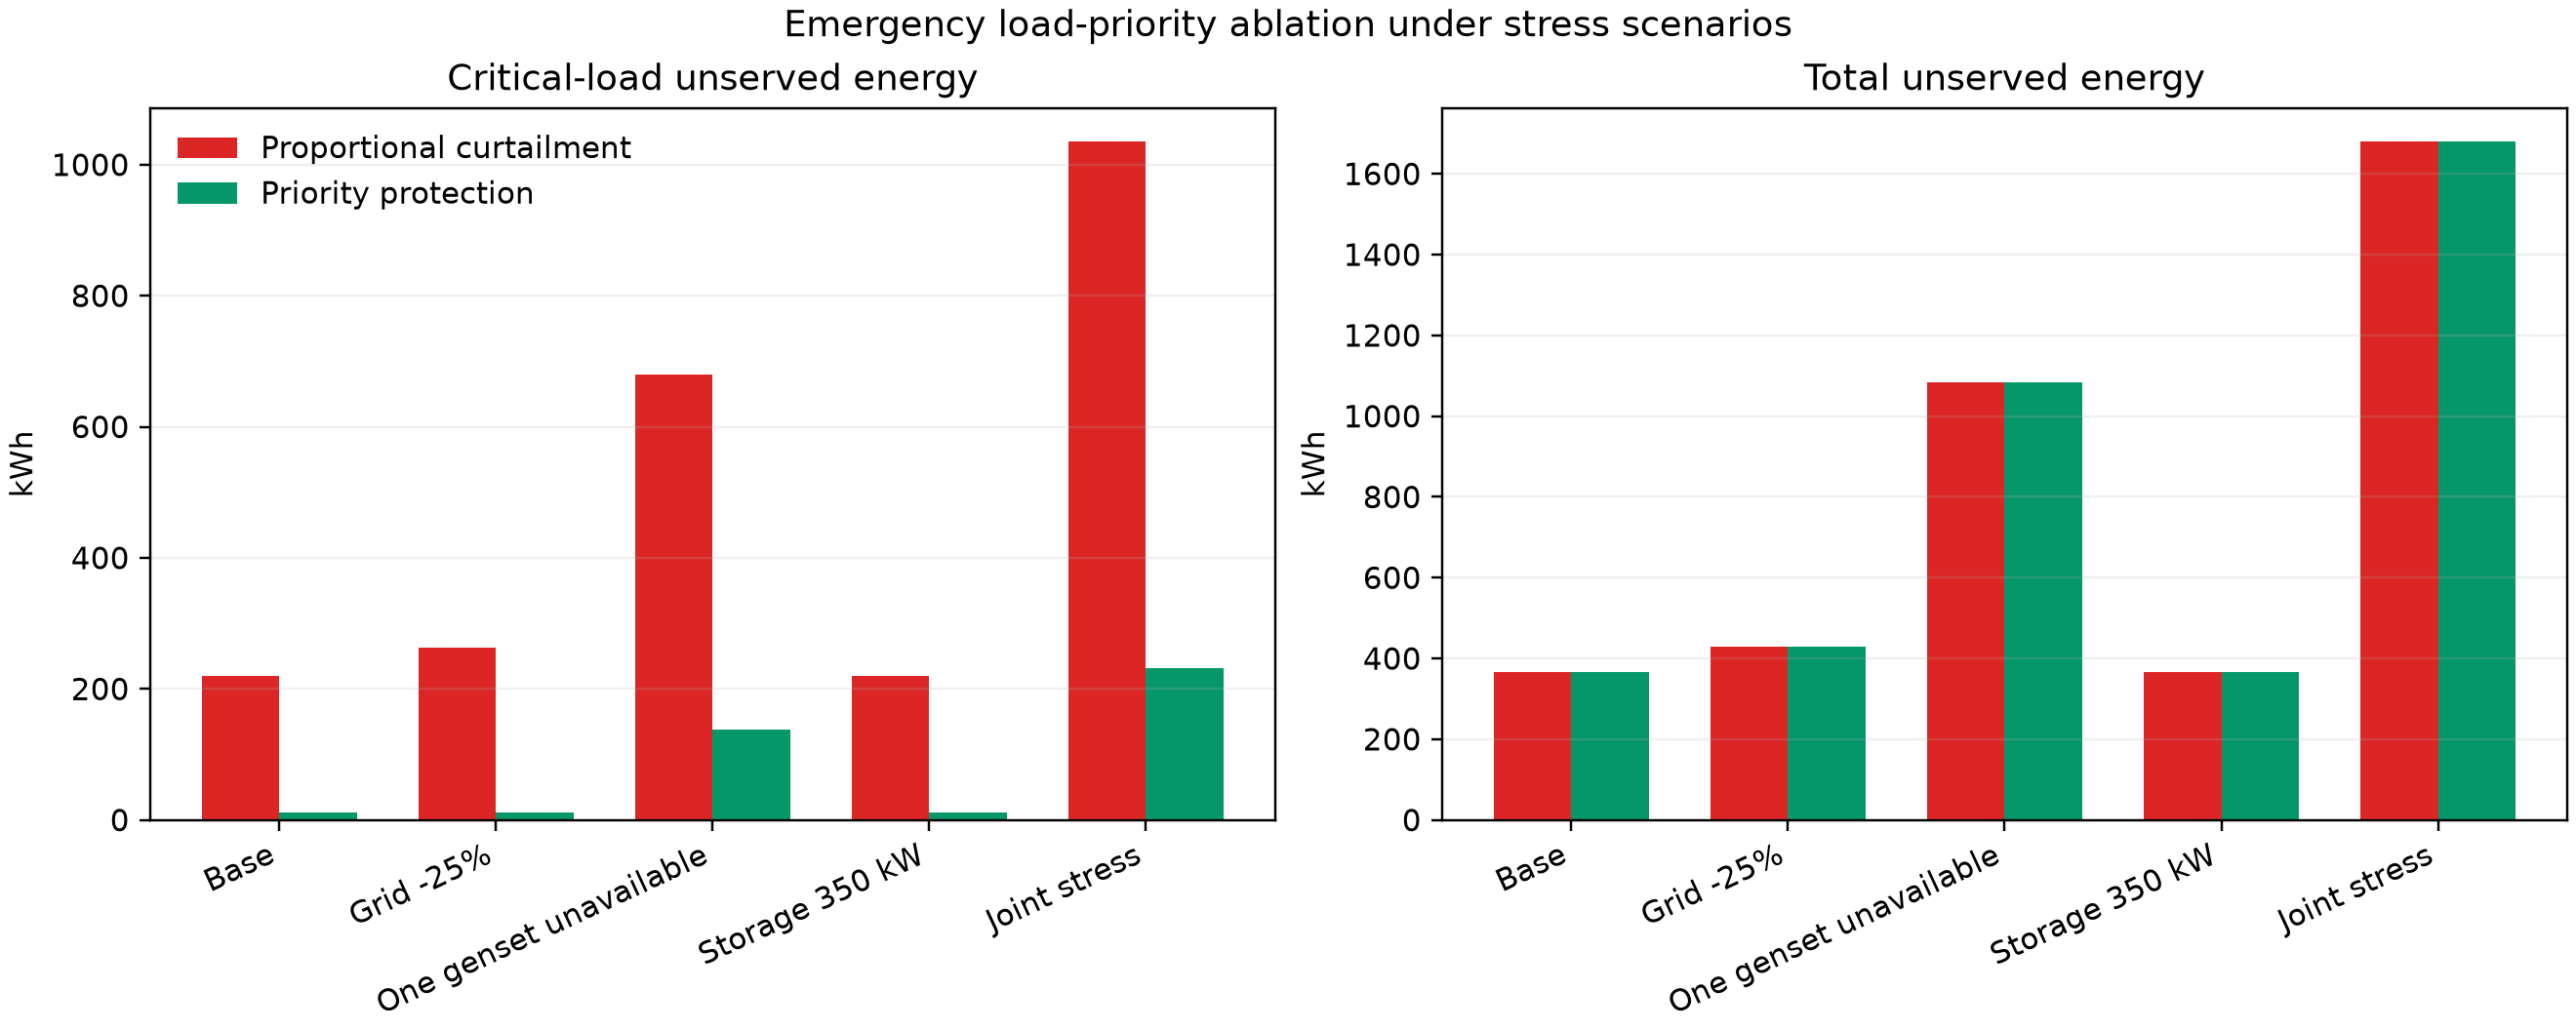
\includegraphics[width=\linewidth,keepaspectratio]{emergency_priority_ablation.png}
\caption{Emergency load-priority ablation}
\label{fig:priority-ablation}
\end{figure}

\begin{table}[!htbp]
\caption{Emergency load priority ablation under stress scenarios}
\label{tab:priority-ablation}
\centering
\footnotesize
\begin{tabular}{@{}
  >{\raggedright\arraybackslash}p{(\linewidth - 8\tabcolsep) * \real{0.1579}}
  >{\raggedleft\arraybackslash}p{(\linewidth - 8\tabcolsep) * \real{0.2105}}
  >{\raggedleft\arraybackslash}p{(\linewidth - 8\tabcolsep) * \real{0.2105}}
  >{\raggedleft\arraybackslash}p{(\linewidth - 8\tabcolsep) * \real{0.2105}}
  >{\raggedleft\arraybackslash}p{(\linewidth - 8\tabcolsep) * \real{0.2105}}@{}}
\toprule
\begin{minipage}[b]{\linewidth}\raggedright
Scenario
\end{minipage} & \begin{minipage}[b]{\linewidth}\raggedleft
Critical unserved: proportional (kWh)
\end{minipage} & \begin{minipage}[b]{\linewidth}\raggedleft
Critical unserved: priority (kWh)
\end{minipage} & \begin{minipage}[b]{\linewidth}\raggedleft
Reduction (kWh)
\end{minipage} & \begin{minipage}[b]{\linewidth}\raggedleft
Total unserved (kWh)
\end{minipage} \\
\midrule
Base & 219.45 & 11.29 & 208.16 & 366.22 \\
Grid derating, 25\% & 263.57 & 11.29 & 252.28 & 430.10 \\
One generator unavailable & 679.87 & 137.84 & 542.03 & 1,083.29 \\
Storage power cap, 350 kW & 219.45 & 11.29 & 208.16 & 366.22 \\
Joint extreme stress & 1,034.90 & 231.16 & 803.75 & 1,679.26 \\
\bottomrule
\end{tabular}
\end{table}

\subsection{Missing-data and combined-stress
diagnostics}\label{missing-data-and-combined-stress-diagnostics}

The missing-data diagnostic increases MAE from 83.94 kW without injected
missingness to 84.33 kW under the moderate condition and 90.66 kW under the
severe condition.

Under a combined disturbance involving 25\% grid derating, one unavailable
generator, a 350 kW storage power cap, a 10 percentage-point SOC bias, a
2.50\% load increase, and a 15 s telemetry delay, priority protection reduces
critical-load unserved energy from 1,034.90 to 231.16 kWh. Total unserved
energy remains 1,679.26 kWh because the allocation layer cannot increase
available supply.

Figure~\ref{fig:joint-stress} shows the detailed joint-extreme trajectory,
complementing the cross-scenario comparison in
Figure~\ref{fig:priority-ablation}.

\begin{figure}
\centering
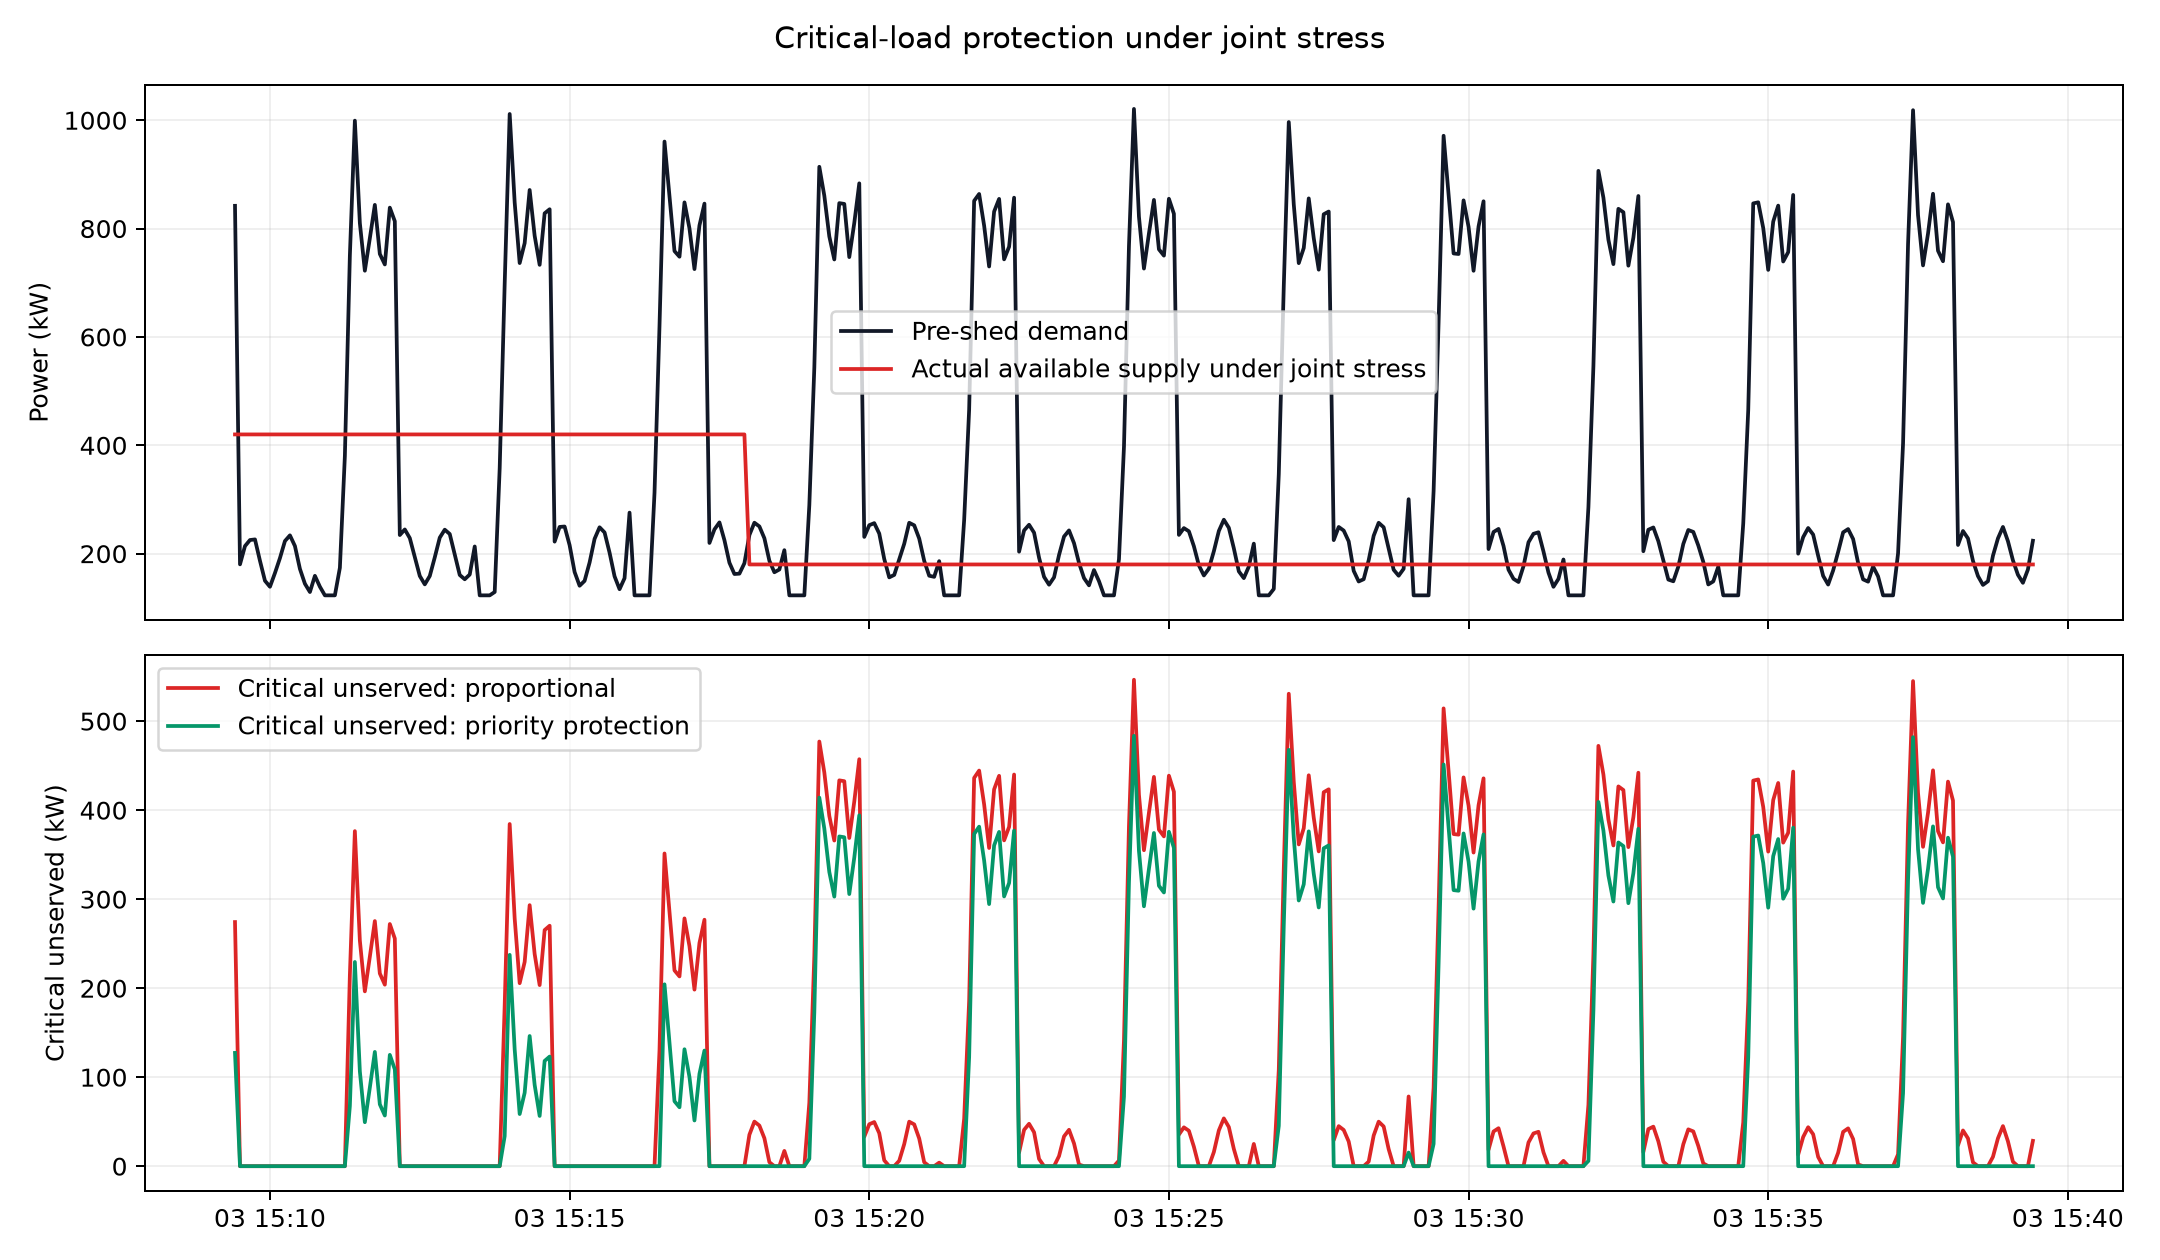
\includegraphics[width=\linewidth,keepaspectratio]{fig07_joint_stress_critical_protection.png}
\caption{Critical-load protection under joint stress}
\label{fig:joint-stress}
\end{figure}

\section{Discussion}\label{discussion}

\subsection{Energy-system performance}\label{energy-system-performance}

Across the 12 frozen simulator seeds, RSS has lower mean EENS than all six
reported alternatives. The three prespecified primary contrasts remain
significant after Holm correction, and their bootstrap intervals exclude zero.
However, four seeds are adverse relative to RB, one is adverse relative to the
point-forecast MILP, and two are adverse relative to the risk-adaptive
residual-CVaR MILP. The mean operating-cost differences are positive in every
primary contrast. The defensible conclusion is therefore a conditional
reliability advantage with higher operating cost, not uniform seed-level or
economic superiority. In particular, the absence of a matched cost-weight
sweep prevents an equal-cost or Pareto-superiority claim.

The public real-data results examine different links in the evidence chain.
Forecast transfer is consistent at 15 and 60 min across eight electrical
series drawn from three dataset families, while the 1-min result is mixed and
includes two significant degradations. Two BESS records support
the sign and coherence of power--SOC relationships used by the controller
model under the stated activity thresholds. Conversely, the two pooled
drilling-process diagnostics challenge the simulator's state-persistence
distribution, although Energistics label coverage limits the comparison. This
combination of supportive and adverse
findings is more informative than treating every public dataset as another
controller benchmark: the data identify which assumptions transfer and which
require recalibration.

\subsection{Operating mechanisms}\label{operating-mechanisms}

The V24 interventions align partially with the proposed mechanism. Removing
generator-first execution or replacing residual scenarios with a point forecast
increases EENS on average, whereas the isolated risk-adaptive CVaR effect is
indistinguishable from zero. The confirmatory full-controller contrast against
risk-adaptive residual-CVaR supports the added reserve--SOC supervisory package,
but the layer contains interacting rules and should not be presented as a
single-rule causal estimate. The fixed supervisor thresholds were not swept,
and no multifactor interaction experiment separates their joint effects.
Priority-based allocation remains a protection
mechanism: it redistributes shortage away from critical loads under severe
stress but cannot reduce total shortage when aggregate supply is fixed.

\subsection{Engineering applicability}\label{engineering-applicability}

Earlier drilling rig studies established the value of rule-based generator
scheduling and battery storage. The present framework adds forecast
uncertainty, discrete multi-generator constraints, explicit storage reserve,
and priority-based protection in a single rolling controller. The resulting
structure is a candidate for evaluation in other industrial
grid--diesel--battery systems with abrupt loads and limited grid capacity. The
public real-data analyses show that the forecasting and storage-variable
interfaces can be exercised on measured records, but they do not establish
transfer of the closed-loop policy.

Deployment requires synchronized total active power, individual generator
states and outputs, battery SOC and power, grid capacity measurements, fuel
consumption, energy prices, and approved load classes. Equipment ramp limits,
minimum up/down times, efficiency curves, startup costs, degradation costs,
and terminal SOC requirements should be replaced with site values. The next
validation step is an external replay with site data followed by
hardware-in-the-loop testing on the intended control platform.

\section{Limitations and reproducibility}\label{limitations-and-reproducibility}

The controller-performance record is generated by one mechanistic simulator
family; synchronized target-rig electrical measurements were not available.
The prospective seeds test stochastic robustness within that simulator, not
transfer across rigs or sites. They do not capture installation-specific
operator actions, protection behavior, or the full communication stack. A
separate heterogeneous-simulation protocol was not complete because one of 12
prespecified units had no eligible stable-drilling window before controller
execution; the remaining 11 units are not used to manufacture a replacement
efficacy conclusion.

The public electrical tests are retrospective cross-domain datasets, not
drilling-rig power. Six series share the REFIT dataset family; UCI is a second
residential source, and the Tsukuba target is reconstructed from microgrid
power channels. The BESS audits are observational and do not compare the native
controllers with RSS. Their reported directional consistency depends on the
frozen activity and $\Delta$SOC thresholds; no threshold or temporal-aggregation
sensitivity was run. OpenCEM
was excluded from confirmation because its intended test period had already
been opened during development. Most importantly, the real drilling-process
records show shorter pooled coarse-state runs than the simulator, but 85.39\%
of Energistics labels are unknown and the state mappings and mixes are not
identical. The result is therefore an adverse diagnostic rather than a direct
state-conditional validation. Until the temporal model is recalibrated and the
controller is rerun, or the mismatch is bounded by an explicit robustness
analysis, the simulation may overstate persistence available to the predictive
controller.

The model is quasi-static and active-power only. Its fixed synchronization delay
does not reproduce diesel-engine speed, voltage build-up, breaker closing,
frequency excursions, converter controls, battery thermal limits, or detailed
aging. SOC-dependent BESS power is represented by a simple linear end-region
derating, and fuel use by a public steady-state piecewise curve. Therefore,
passing the constraint audit is not evidence of electrical stability or safety.
The emergency load classes and all equipment and economic parameters require
site-specific approval and calibration.

The cost model is a configured proxy containing grid energy, diesel fuel,
linear storage throughput, and a 5-yuan start-command term. It excludes demand
charges, nonlinear battery aging, maintenance, and site-calibrated hot/cold
start wear. The reported start quantity is a model-level command count over
three disjoint stress windows, not a field cold-start rate. The 12-seed sample
also limits inferential resolution and remains conditional on one simulator
family. No confirmatory startup-delay, cost-weight, supervisor-threshold, or
BESS-size sweep is available, so the parameter choices and higher switching
rate should not be interpreted as economically optimized.

The research implementation treats a missing or over-time optimization result
as a technical-gate failure; it does not silently substitute a successful
trajectory. No hold-last-command or rule-based switchover was evaluated.
Deployment would additionally require a certified, constraint-safe fallback
policy and timing tests on the intended controller hardware; the observed
development-platform latency distribution establishes neither industrial
real-time certification nor fail-safe behavior.

The source artifacts, configurations, result manifests, and analysis scripts
are versioned locally. Frozen configuration hashes, source hashes, failed-run
records, and the 24 real-data forecast outputs are retained in the evidence
ledger. The permitted V24/V28 additions must be included in an updated archival
reproducibility package before submission of the revised manuscript and
artifact; until then, public v1.0.0 is incomplete for the reported results.
Raw third-party datasets remain
subject to their original licenses.

\section{Conclusions}\label{conclusions}

This paper evaluated whether causal forecast information can be used to
coordinate storage reserve with model-reachable diesel generation during abrupt
drilling-load transitions. The reserve--SOC supervisor combines forecast-error
scenarios with CVaR dispatch, integer generator commitment, and SOC hysteresis
within a grid--diesel--battery power-system model.

Across 12 frozen simulation seeds, RSS reduces mean EENS by 5.24 kWh relative
to rule-based control, 15.59 kWh relative to point-forecast MILP, and 5.49 kWh
relative to risk-adaptive residual-CVaR control. All three intervals exclude
zero, and all three exact tests remain significant after Holm correction. Mean realized operating
cost is 153.83--280.17 yuan higher, so the result is a reliability--cost
trade-off and does not establish equal-cost or Pareto superiority. Component
interventions support residual scenarios, generator-first execution, and the
supervisory package; they do not support an
independent reliability effect for adaptive CVaR.

Public real measurements add bounded component evidence without closing the
controller-validation gap. Eight electrical series from three dataset families
support cross-domain forecasting most consistently at 15 and 60 min, and two
BESS records support coherent power--SOC behavior under frozen eligibility
rules. Pooled diagnostics from two drilling records, however, challenge the
simulator's state-persistence distribution; the high unknown-label fraction in
Energistics precludes a like-for-like calibration claim. Within these
boundaries, the results support
coordinating storage reserve with forecast uncertainty and model-reachable generator
capacity in the frozen simulation. Site-specific electrical replay,
real-data-informed temporal recalibration, and hardware-in-the-loop testing are
required before drawing field-performance conclusions.
